\documentclass[../main.tex]{subfiles}
\begin{document}
%\chapter{Results}\label{ch:A}
This chapter focuses on the effects on the performance of the quantum annealing algorithm upon adding the antiferromagnetic trigger to the original Hamiltonian. Unlike the case of the ferromagnetic trigger, for the antiferromagnetic trigger the strength parameter, $g$ in Eq.~(\ref{eq:b12}) plays a more decisive role than merely controlling the extent by which the minimum gap is enlarged. The antiferromagnetic trigger alters the energy spectra, the minimum energy gaps, and the number of anti-crossings between the ground and first excited energy state of the Hamiltonian, depending on the strength with which it is added, as well as on the problem itself. We shall begin by observing the effects of adding the antiferromagnetic trigger to the original Hamiltonian, for the three chosen problems. The following sections will then showcase the role that the strength parameter $g$ plays.

\section{The Selected Problems}
Contrary to the systematic effects of adding the ferromagnetic trigger, where adding the trigger always enlarges the minimum energy gap, and both larger minimum energy gaps and longer annealing times result in a higher success probability, the effects of adding the antiferromagnetic trigger are very specific to the problem at hand, and the chosen annealing time. This is a consequence of many non-adiabatic mechanisms involved in improving the success probability as well.\\

Let us begin by considering problem 733 again, which was found to have a large success probability for the original Hamiltonian. \\

Table~(\ref{tab:a1}) shows a comparison of the success probabilities $p$, and minimum energy gaps $\Delta_{min}$ between the original Hamiltonian and the Hamiltonian after adding the antiferromagnetic trigger with different strengths to problem 733.
\begin{figure}
\centering 
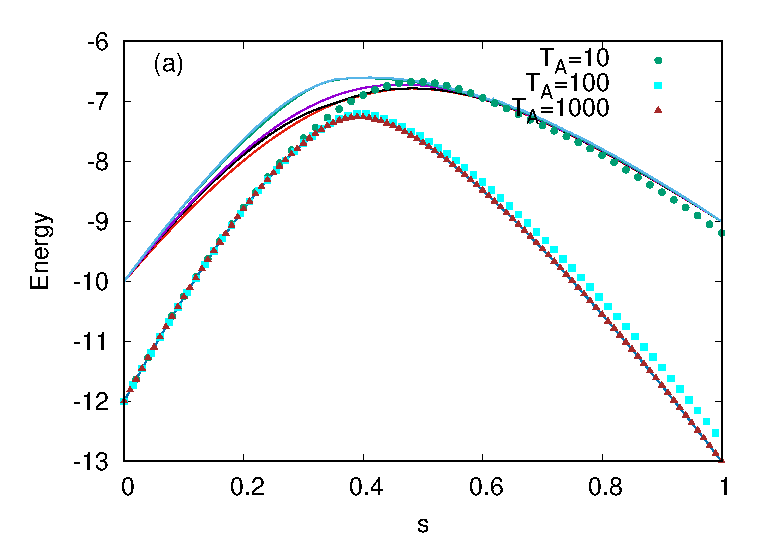
\includegraphics[scale=0.8]{733_s12_A_g0.eps}
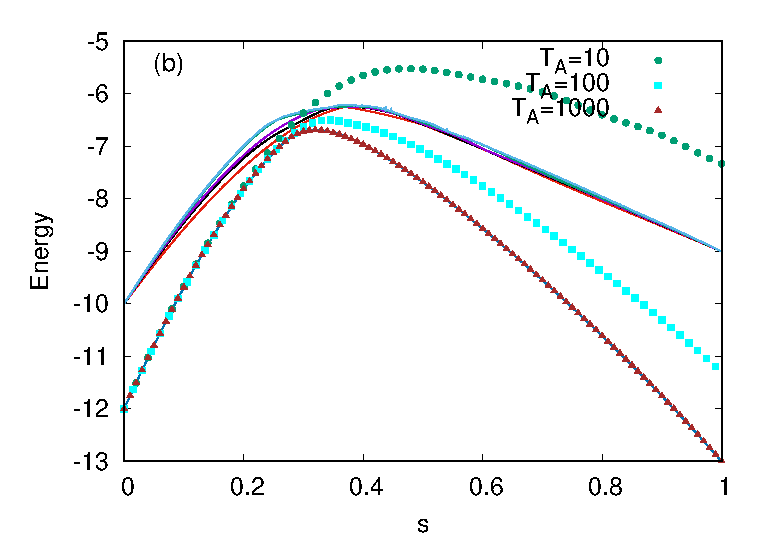
\includegraphics[scale=0.8]{733_s12_A_g1.eps}
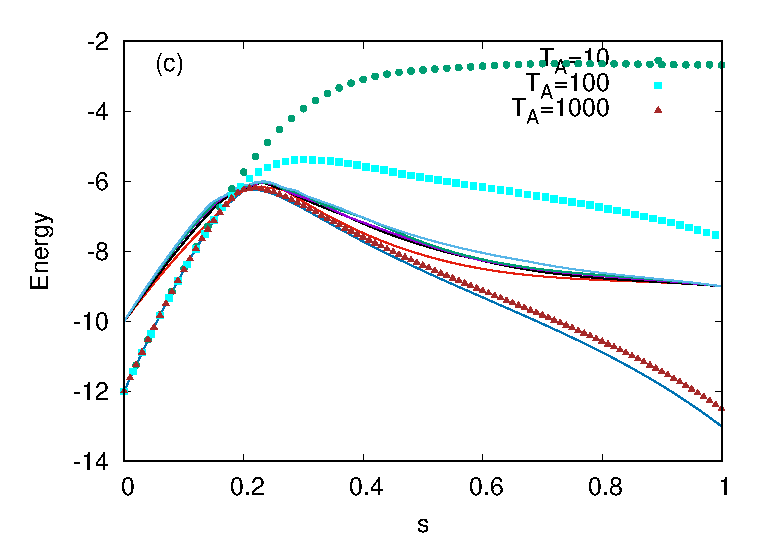
\includegraphics[scale=0.8]{733_s12_A_g2.eps}
\caption{The energy spectrum and energy expectation values for the instantaneous state of problem 733, after adding the antiferromagnetic trigger. (a): $g$=0.5; (b): $g$=1; (c): $g$=2.}
\label{fig:a1}
\end{figure}
Figure~(\ref{fig:a1}) shows the energy spectra and the energy expectation values for the instantaneous state corresponding to the three annealing times, after adding the antiferromagnetic trigger to the Hamiltonian with strengths 0.5, 1 and 2.

\begin{table}[H]
\centering
\renewcommand{\arraystretch}{1.5}
\begin{tabular}{|c|c|c|c|c|}
\hline 
Problem 733 & Original Hamiltonian & Trigger=A, $g$=0.5 & Trigger=A, $g$=1 & Trigger=A, $g$=2 \\ 
\hline 
$\Delta_{min}$ & 0.4407 & 0.3070 & 0.1349 & 0.0020 \\ 
\hline 
$p$($T_A$=10) & 0.3444 & 0.1446 & 0.0279 & 1.271 $\times 10^{-4}$ \\ 
\hline 
$p$($T_A$=100) & 0.9944 & 0.9117 & 0.5747 & 0.0273 \\ 
\hline 
$p$($T_A$=1000) & 0.9999 & 0.9999 & 0.9999 & 0.8761 \\ 
\hline 
value of $s$ at $\Delta_{min}$ & 0.459 & 0.367 & 0.282 & 0.254 \\ 
\hline
Number of anti-crossings & 1 & 1 & 1 & 3 \\
\hline
\end{tabular} 
\caption{A comparison of the minimum energy gaps and the success probabilities for problem 733, between the original Hamiltonian and the Hamiltonian with antiferromagnetic trigger (A) of different strengths. The minimum gaps become successively smaller as the strength of the antiferromagnetic trigger is increased. The success probabilities are decreased as a result. The value of $s$ corresponding to the position of the minimum gap also becomes smaller.}
\label{tab:a1}
\end{table}
As can be noted from the table, the minimum energy gap decreases upon adding the antiferromagnetic trigger, and this decrease becomes larger as the strength of the trigger is increased. Consequently, the success probabilities after adding the trigger are found to be decreasing as well. The value of annealing parameter $s$ at the position of minimum gap also becomes smaller with increasing strength of the trigger.\\
Additionally, a new feature observed as a result of adding the antiferromagnetic trigger (compared to the effects of adding the ferromagnetic trigger) is the change in the number of anti-crossings between the ground and the first energy state. For strength $g$=2, the number of energy anti-crossings increases to 3, while it remains unchanged for $g$=0.5 and $g$=1. Moreover, when the antiferromagnetic trigger is added with strength 2, the energy spectrum changes significantly (in terms of the number of the energy anti-crossings between the energy levels of the spectrum and the time duration for which the two lowest lying energy levels remain in close proximity) in comparison to the original spectrum (see Fig.~\ref{fig:o2}), as can be seen more clearly in the inset of Fig.~(\ref{fig:a1}(c)).\\

Next, let us consider problem 950 that had a small success probability in the absence of any triggers. Figure~(\ref{fig:a4}) shows the energy spectrum and the energy expectation values for the instantaneous state corresponding to the three annealing times, after adding the antiferromagnetic trigger to the Hamiltonian with strengths 0.5, 1 and 2. 


\begin{figure}
\centering 
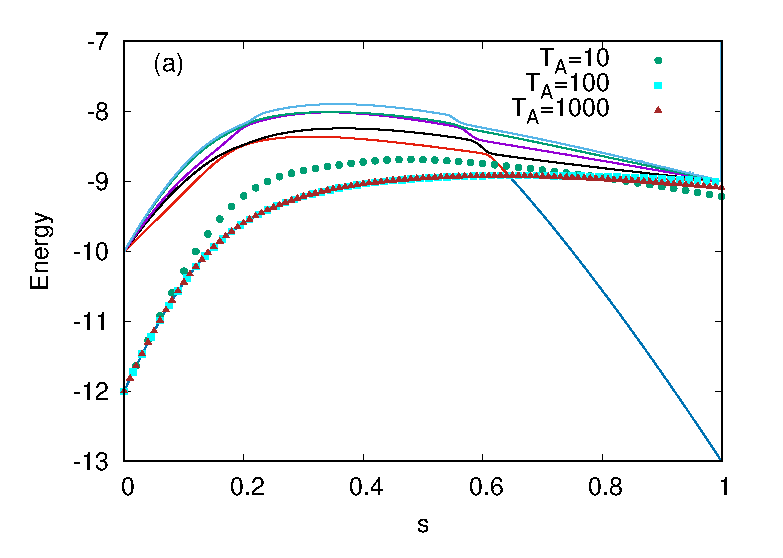
\includegraphics[scale=0.8 ]{950_s12_A_g0.eps}
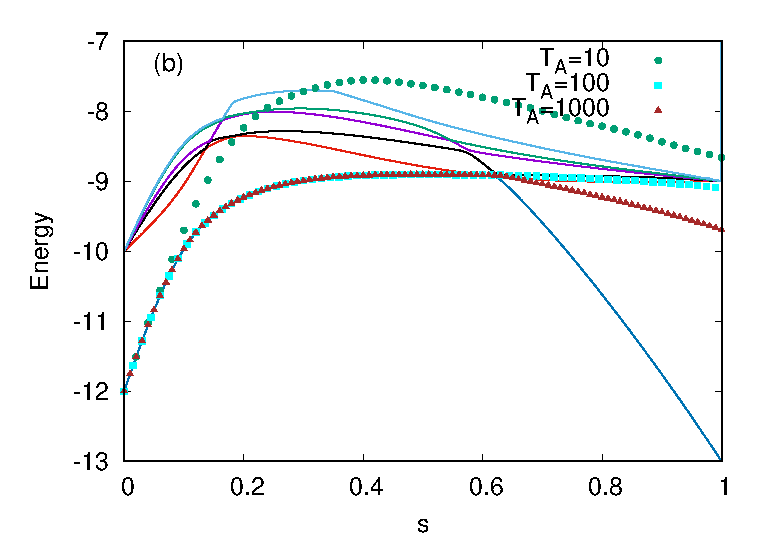
\includegraphics[scale=0.8 ]{950_s12_A_g1.eps}
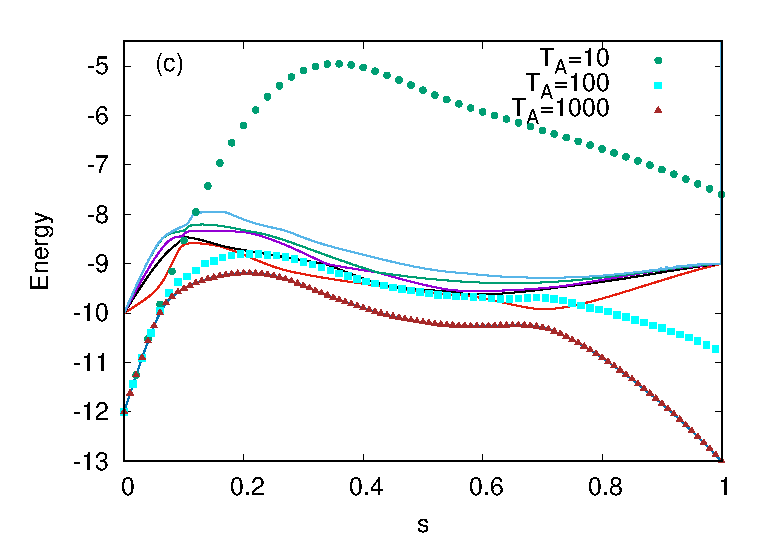
\includegraphics[scale=0.8 ]{950_s12_A_g2.eps}
\caption{The energy spectrum and energy expectation values for the instantaneous state of problem 950, after adding the antiferromagnetic trigger. (a): $g$=0.5; (b): $g$=1; (c): $g$=2. }
\label{fig:a4}
\end{figure}
For this case, Table~(\ref{tab:a2}) shows a comparison of the minimum energy gaps, and success probabilities corresponding to different strengths for the antiferromagnetic. 

\begin{table}[H]
\centering
\renewcommand{\arraystretch}{1.5}
\begin{tabular}{|c|c|c|c|c|}
\hline 
Problem 950 & Original Hamiltonian & Trigger=A, g=0.5 & Trigger=A, g=1 & Trigger=A, $g$=2 \\ 
\hline 
$\Delta_{min}$ & 0.0312 & 0.0130 & 0.0019 & 0.1784 \\ 
\hline 
$p$($T_A$=10) & 2.343 $\times 10^{-4}$ & 0.0567 & 0.0017 & 0.0071\\ 
\hline 
$p$($T_A$=100) & 0.0146 & 0.0022 & 0.0239 & 0.4468 \\ 
\hline 
$p$($T_A$=1000) & 0.1362 & 0.0228 & 0.1729 & 0.9999 \\ 
\hline 
value of $s$ at $\Delta_{min}$ & 0.665 & 0.644 & 0.601 & 0.263 \\ 
\hline 
Number of anti-crossings & 1 & 1 & 2 & 3 \\
\hline
\end{tabular} 
\caption{A comparison of the minimum gaps and the success probabilities for problem 950, between the original Hamiltonian and the Hamiltonian with the antiferromagnetic trigger (A) of different strengths. The minimum gap becomes small for $g$=0.5, and even smaller for $g$=1, while it becomes even larger than the original minimum energy gap for $g$=2. The value of $s$ corresponding to the position of the minimum gap becomes smaller with increasing strength of the trigger.}
\label{tab:a2}
\end{table}


The minimum energy gaps decrease with respect to the original minimum gaps, upon adding the trigger with strengths 0.5, and 1. However, the success probability for $T_A$=10 after adding the antiferromagnetic trigger with $g$=0.5 and $g$=1, is larger compared to that of the original Hamiltonian, owing to different reasons.\\

Since upon adding the antiferromagnetic trigger with strength 0.5, the minimum energy gap becomes smaller, the annealing time of $T_A$=10 is so short that the state of the system transits to the first excited state even before the minimum gap anti-crossing. Upon approaching the minimum gap anti-crossing the system state shifts some of the amplitude back to the ground state, increasing the success probability in this case (see Fig.~\ref{fig:a4}(a)). However, for the original Hamiltonian the gap is not large enough for $T_A$=10 for the state to jump to the first excited state before the minimum energy gap (see Fig.~\ref{fig:o3}). The state therefore stays close to the first excited state after passing the anti-crossing.\\
Furthermore, for annealing times $T_A$=100 and $T_A$=1000, the system state transitions only at the minimum gap anti-crossing and closely follows the second and first excited states respectively. The overlap with the ground state decreases, and therefore the success probability in both these cases also reduces.\\

In case of adding the antiferromagnetic trigger with strength 1, the first energy anti-crossing is small enough for $T_A$=10 to shift the system state to the first excited state. Quickly after transitioning to the first excited state, the system state shifts to the higher energy levels (see Fig.~\ref{fig:a4}(b)). Since the state of the system is a superposition of many energy eigenstates, the final system state has small, yet finite overlap with the ground state. In the original Hamiltonian, however, the system state shifts to the first excited state at the anti-crossing and stays there. Therefore, the overlap with the ground state becomes negligible (see Fig.~\ref{fig:o3}).\\

By choosing the strength to be 2, the minimum energy gap for this problem becomes larger than the original minimum energy gap, while the number of anti-crossings between the ground and the first excited state increases to 3. The success probability in this case is larger than the original success probability for all the annealing times. For $T_A$=10, the state of the system shifts to the first excited state at first energy anti-crossing, and then quickly shifts to a superposition state of the higher energy states (due to the proximity of the higher energy levels as result of adding the trigger). In this particular case, this results in a larger overlap with the ground state compared to the case of the state closely following the first excited state after reaching the only energy anti-crossing in case of the original problem (see Fig.~\ref{fig:o3}).\\
Thus, in this case adding the antiferromagnetic trigger with different strengths can decrease or increase the minimum energy gap, thus affecting the success probabilities by different mechanisms.

For $T_A$=100, the state starts transitioning to the first excited state only as it approaches the second energy anti-crossing. The state does further shifts to higher energy levels, but comes back to the first excited state before the third energy anti-crossing. At the third anti-crossing some of the amplitude of the wave function shifts to the ground state again, and therefore the success becomes larger than the original problem. 


Finally, for $T_A$=1000, the annealing time and the minimum energy gap is large enough for the system to always stay close to the ground state, hence the larger success probability.\\

Lastly, Fig.~(\ref{fig:a7}) shows the energy spectra and the energy expectation values for the state for problem 528, after adding the antiferromagnetic trigger with strengths 0.5, 1 and 2. 


\begin{figure}
\centering 
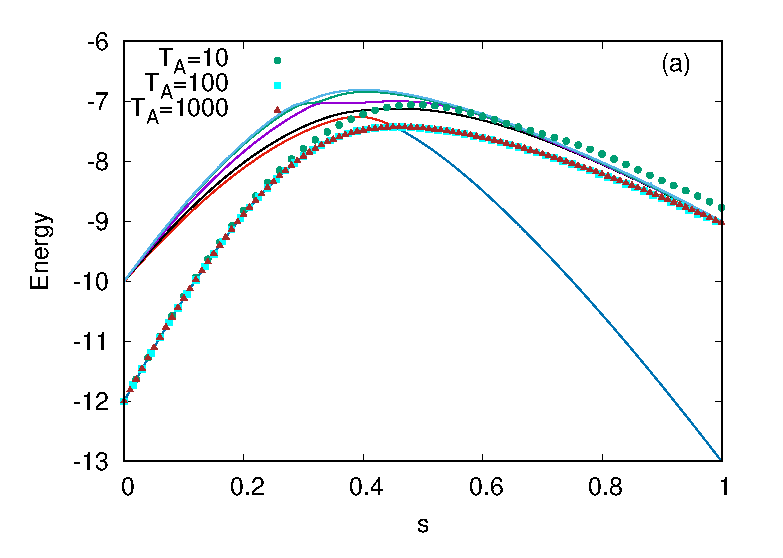
\includegraphics[scale=0.8]{528_s12_A_g0.eps}
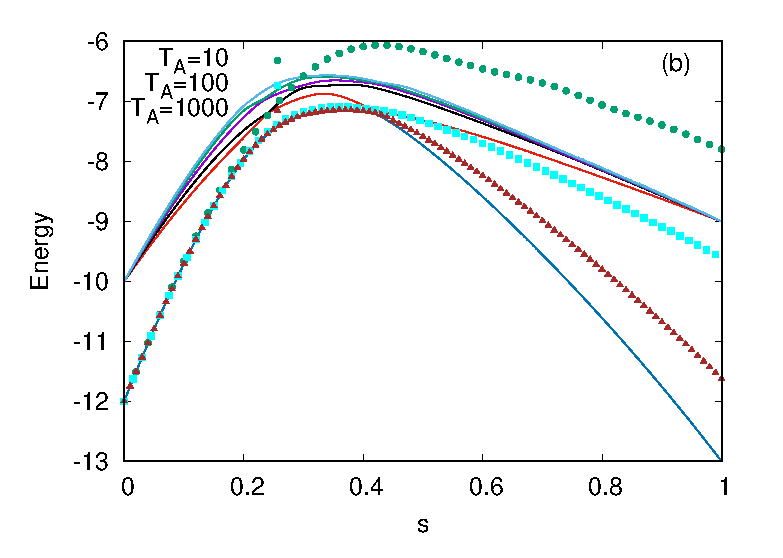
\includegraphics[scale=0.8]{528_s12_A_g1.eps}
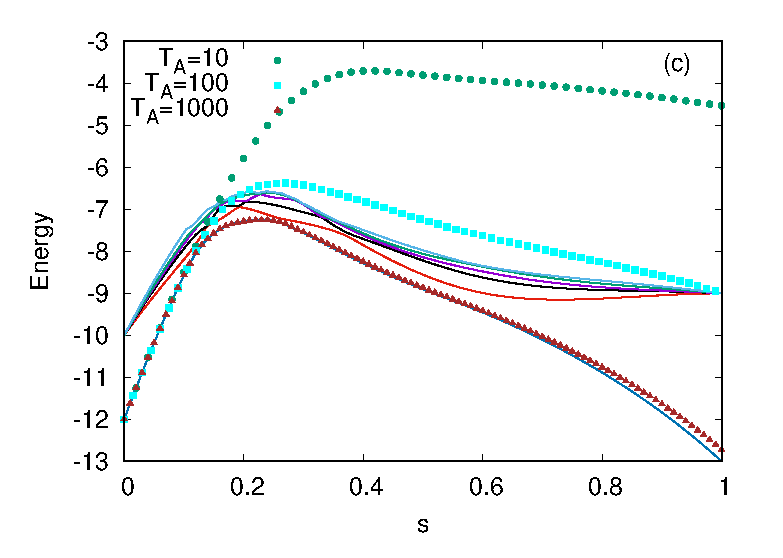
\includegraphics[scale=0.8]{528_s12_A_g2.eps}
\caption{The energy spectrum and energy expectation values for the instantaneous state of problem 528, after adding the antiferromagnetic trigger. (a): $g$=0.5; (b): $g$=1; (c): $g$=2.}
\label{fig:a7}
\end{figure}

Table~(\ref{tab:a3}) shows a comparison of the minimum energy gaps, and success probabilities (corresponding to different annealing times) between the original Hamiltonian and the Hamiltonian after adding the antiferromagnetic trigger with different strengths for problem 528. 

\begin{table}[H]
\centering
\renewcommand{\arraystretch}{1.5}
\begin{tabular}{|c|c|c|c|c|}
\hline 
Problem 528 & Original Hamiltonian & Trigger=A, $g$=0.5 & Trigger=A, $g$=1 & Trigger=A, $g$=2 \\ 
\hline 
$\Delta_{min}$ & 0.1573 & 0.0049 & 0.0562 & 0.1008 \\ 
\hline 
$p$($T_A$=10) & 0.1577 & 0.0573 & 0.0368 & 4.21 $\times 10^{-5}$\\ 
\hline 
$p$($T_A$=100) & 0.5199 & 0.0120 & 0.1517 & 0.0480 \\ 
\hline 
$p$($T_A$=1000) & 0.9992 & 0.0071 & 0.6565 & 0.9313 \\ 
\hline 
value of $s$ at $\Delta_{min}$ & 0.514 & 0.454 & 0.418 & 0.256 \\ 
\hline 
Number of anti-crossings & 1 & 1 & 3 & 4 \\
\hline
\end{tabular} 
\caption{A comparison of the minimum energy gaps and the success probabilities for problem 528, between the original Hamiltonian and and the Hamiltonian with antiferromagnetic trigger (A) of different strengths. The minimum energy gaps after adding the trigger are smaller than the original minimum gap, for all the values of $g$. They however become large upon increasing the strength of the antiferromagnetic trigger. The value of $s$ corresponding to the position of the minimum gap becomes smaller with increasing strength of the trigger.}
\label{tab:a3}
\end{table}

For this problem, adding the antiferromagnetic trigger makes the minimum energy gaps smaller than the original gap, for all the three $g$ values. The gaps however increase with increasing the strength of the trigger. The original success probabilities, for all annealing times, are therefore larger than the resulting success probabilities upon adding the triggers with different $g$. Additionally, for $T_A$=100, 1000, the success probabilities become larger when the antiferromagnetic trigger is added with strength 1 compared to when added with strength 0.5, as the minimum energy gap for the former is larger. For $T_A$=10, and both $g$=0.5 and $g$=1 cases, the system state transitions to the first excited state prior to the first energy anti-crossing. This is followed by the state shifting to higher energy levels soon after. Since the energy spectrum becomes more complex (in terms of the number of anti-crossings between the higher energy states and their proximity) as the strength of the trigger is increased, the system state shifts farther away from the ground state. For this problem, the state of the system with $g$=0.5 ends in a superposition state with a higher overlap with the ground state than the final state of the system with $g$=1.

Although the gap becomes even larger with $g$=2, the success probability in this case is smaller compared to the case with $g$=1 for $T_A$=10 and $T_A$=1000. This can be explained by observing that adding the antiferromagnetic trigger with $g$=2 changes the energy spectrum of the Hamiltonian even more drastically. Not only do the number of energy anti-crossings between the ground and the first excited state increase to 4, the higher lying energy levels also become more involved and have a larger number of crossings and anti-crossings. Therefore, as annealing times $T_A$=10 and $T_A$=100 are not large enough for the state to stay close to the ground state upon reaching the first energy anti-crossing, the system state settles even farther away from the ground state as compared to the $g$=1 case. The overlap of the  resulting state with the ground state is even smaller and hence, the success probability for $g$=2 for $T_A$=10 is negligible. As the annealing time is increased further to $T_A$=1000, the minimum energy gap becomes large enough to keep the state of the system close to the ground state, and the success probability becomes comparable to the original success probability.

Thus adding the antiferromagnetic trigger is capable of both enlarging and reducing the minimum energy gap, and therefore capable of improving the success probability by making the evolution more close to adiabatic, or by non-adiabatic mechanisms. It therefore becomes essential to study the effects of the strength parameter on altering the minimum energy gaps, and thereby the choice of the annealing time on the success probability.
 
\section{Trigger Strength g=0.5}
This section will showcase the effects of adding the antiferromagnetic trigger to  all the original Hamiltonians from the set of 12 spin problems, with strength 0.5. For each problem, the annealing time was chosen to be 10, 100 and 1000. 

As a measure of quantifying the performance with respect to the original Hamiltonian, the relative success probability was defined as the ratio of the success probability upon adding the antiferromagnetic trigger ($p^A$) to the original success probability ($p^O$). Figure~(\ref{fig:a10}) shows the distribution of the relative success probability for annealing times of 10, 100 and 1000, with the strength of the trigger Hamiltonian chosen to be 0.5.

\begin{figure}
\centering 
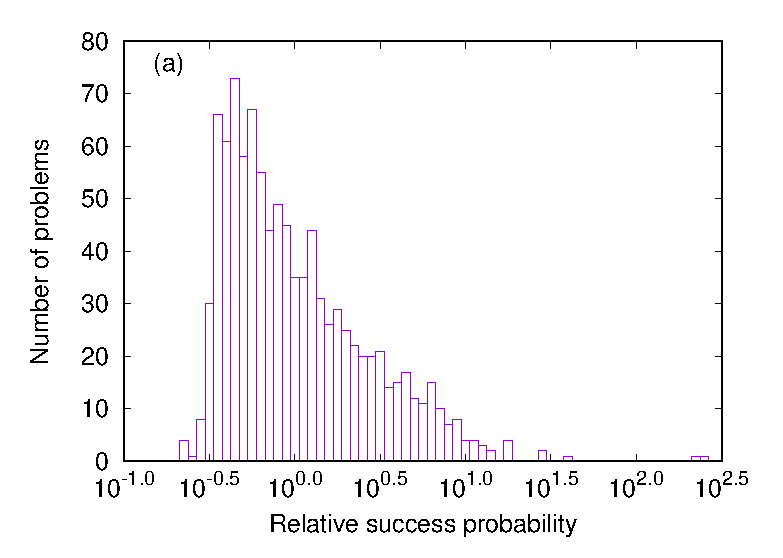
\includegraphics[scale=0.8]{A_T10_g0.eps}
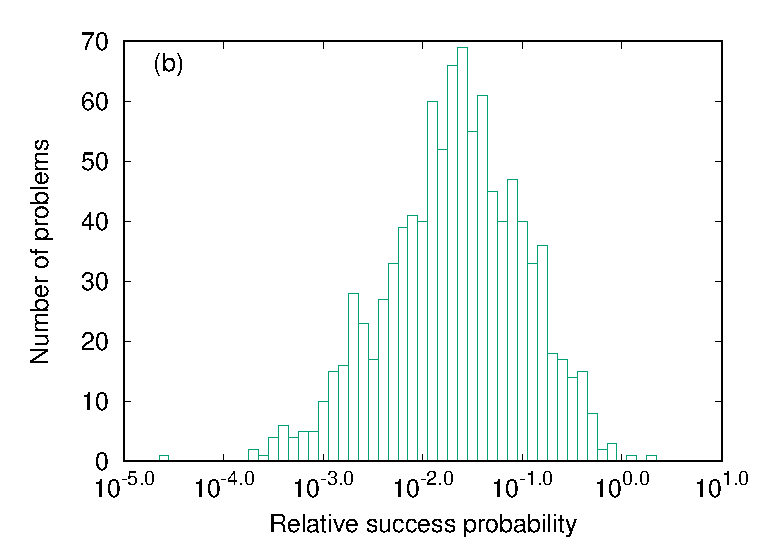
\includegraphics[scale=0.8]{A_T100_g0.eps}
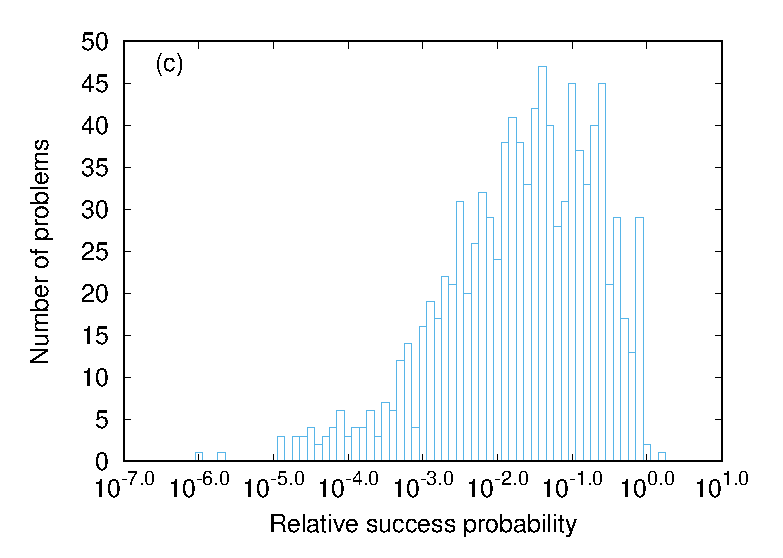
\includegraphics[scale=0.8]{A_T1000_g0.eps}
\caption{Distribution of the relative success probability $p^A/p^O$ for $g$=0.5.(a): $T_A$=10; (b): $T_A$=100; (c): $T_A$=1000.}
\label{fig:a10}
\end{figure}


For an annealing time $T_A$=10, 439 problems of the set are improved after including the antiferromagnetic trigger with $g$=0.5. On increasing the annealing time to 100 and 1000, the number of cases with improved success probability drops to 2 for both the cases. Furthermore, the largest value of the relative success ratio is a little more than 250 for $T_A$=10, while it reduces to 1.995 for $T_A$=100, and to 1.585 for $T_A$=1000. In order to understand the reasons for this decrease in the relative success ratio on increasing the annealing time, the minimum energy gaps of all the problems were calculated before and after adding the trigger. Figure~(\ref{fig:a13}) shows a plot of the minimum energy gaps after adding the antiferromagnetic trigger ($\Delta_{min}^A$) with $g$=0.5, against the original minimum energy gaps ($\Delta_{min}^O$). The points lying above the line $\Delta_{min}^O=\Delta_{min}^A$ represent the problems for which the energy gaps increase after adding the trigger. (See Fig.~(\ref{fig:ap2}) in the appendix for the similar minimum energy scatter plot for the 8-spin problems for all the values of $g$.)
\begin{figure}[H]
\centering 
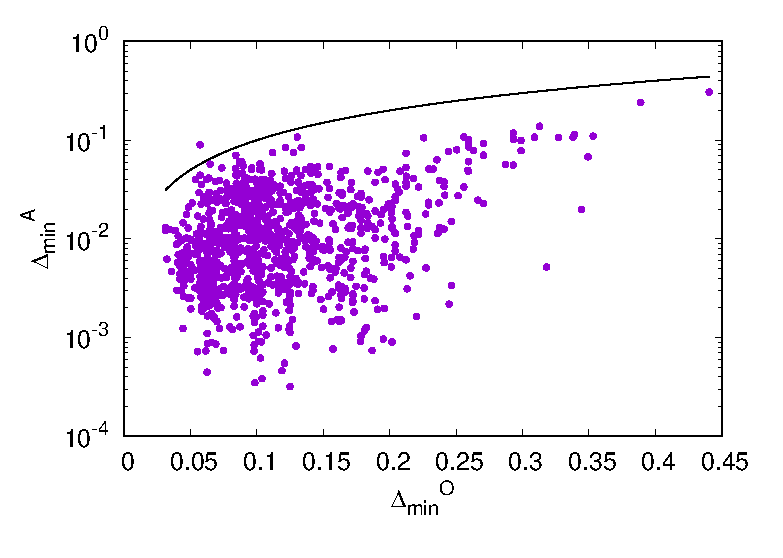
\includegraphics[scale=0.8]{MinGap_A_g0.eps}
\caption{A plot of the minimum energy gaps after adding the antiferromagnetic trigger with $g$=0.5 ($\Delta_{min}^A$), with the original minimum energy gaps ($\Delta_{min}^O$). For 999 problems of the minimum energy gap was found to have decreased after adding the antiferromagnetic trigger.}
\label{fig:a13}
\end{figure}
As is clear from Fig.~(\ref{fig:a13}), for 999 problems, the minimum energy gaps reduce after adding the antiferromagnetic trigger with strength 0.5. It was also found that 923 problems still have a single anti-crossing between the ground and the first excited state, while for the other 77 problems, it increases to 2.\\
For some cases with small original minimum energy gaps and short annealing time of $T_A$=10, non-adiabatic evolution of the state results in a larger overlap of the final state with the ground state. Some of these mechanisms can be the state deviating from the ground state even before the anti-crossing and transferring some of the amplitude back to the ground state, or the presence of 2 sufficiently small and comparable anti-crossings, or a coincidental larger overlap of the final state with the ground state as a consequence of being a superposition state. Thus, when the annealing time is increased to 100 or 1000, the state shifts to the first excited state only at the anti-crossing, and follows it closely. This explains the drop in the percentage of improved cases upon increasing the annealing time after adding the trigger. 


\begin{figure}
\centering 
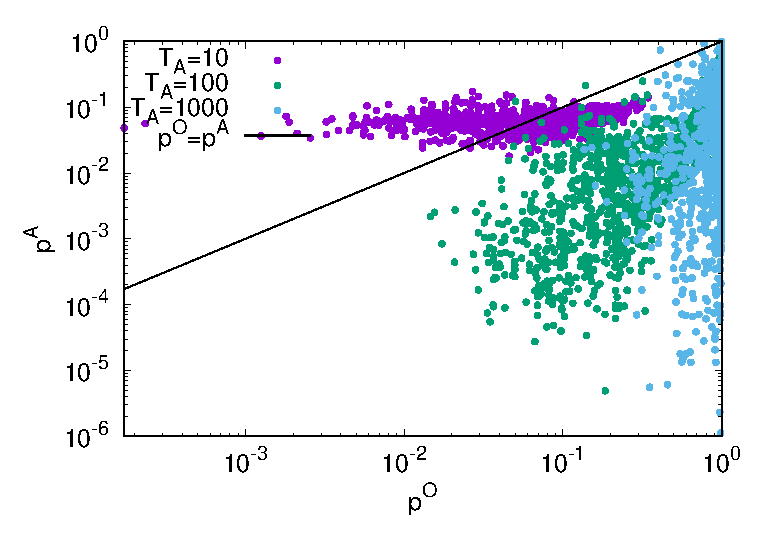
\includegraphics[scale=0.8]{ProbScat_g0.eps}
\caption{A plot of the success probabilities after adding the antiferromagnetic trigger with $g$=0.5 ($p^A$), with the original success probabilities($p^O$) for annealing time 10, 100 and 1000.}
\label{fig:a14}
\end{figure}

To obtain an estimate of the difficulty of the affected problems, Fig.~(\ref{fig:a14}) shows a scatter plot of the success probabilities after adding the trigger against the original success probabilities, for the three annealing times. (See Fig.~\ref{fig:ap4} in the appendix for the similar success probability scatter plot for the 8-spin problems for all the values of $g$.) The points lying above the line $p^O=p^A$ represent the cases with improved success probability after including the antiferromagnetic trigger. It should be noted that the 439 problems improved by adding antiferromagnetic trigger for $T_A$=10, are the ones that have a relatively smaller original success probabilities (harder problems with smaller minimum energy gaps). This suggests that the mechanisms leading to an improvement in the success probability are mostly non-adiabatic in this case.\\
It should also be noted that for $T_A$=100 and $T_A$=1000, the original success probabilities are already quite high, giving way to another reason for the decrease in the relative success probability with increasing annealing time. \\

For both $T_A$=100 and $T_A$=1000 problem number 402 and 709 have a larger relative success ratio upon adding the antiferromagnetic trigger with $g$=0.5. Problem 402 corresponds to the only case where the minimum energy gap increases after adding the trigger, explaining the reason for the increase in the success probability.\\
For problem 709, Fig.~(\ref{fig:a15}) shows the energy gap between the ground state and the first excited state of the Hamiltonian (as a function of the annealing parameter $s$), before and after adding the antiferromagnetic trigger. The inset of the figure also shows the energy gaps for some other problems after adding the trigger. As can be observed from the figure, the shape of the curve after adding the antiferromagnetic trigger to problem 709 is different than both the curve for the original Hamiltonian of this problem and the other problems. The slope in this case, unlike the other cases, is not symmetric about the minimum gap value. While comparing the success probabilities across different problems (and assuming $p=1-\exp({-{-T {\Delta}^2/c}})$), the slope ($c$) for each problem was supposed to have a similar value, and only changes in the minimum gaps were accounted for. Since this assumption breaks down for this case, the Landau-Zener formula no longer holds good for this problem.\\

\begin{figure}
\centering 
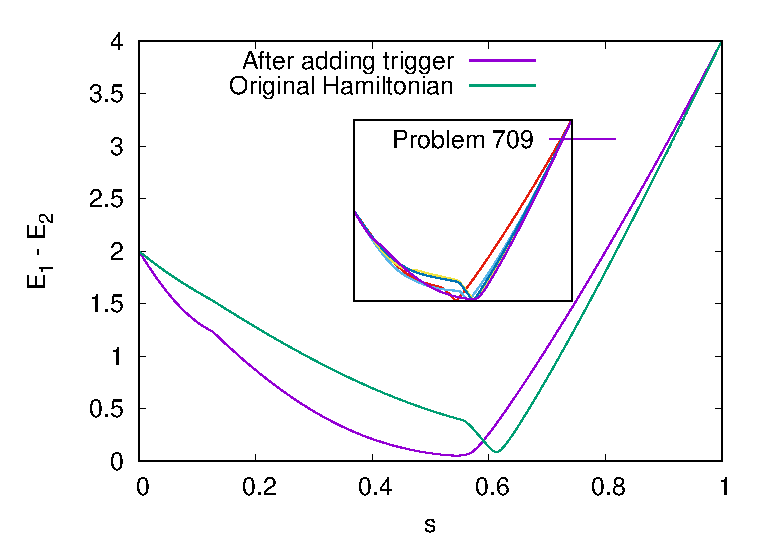
\includegraphics[scale=0.8 ]{Mingap_709_g0_A.eps}
\caption{A comparison of the minimum energy gaps between the two lowest energy levels as a function of the annealing parameter $s$, in the absence and presence of the antiferromagnetic trigger with $g$=0.5. The inset shows a comparison with some other problems after adding the trigger.}
\label{fig:a15}
\end{figure}

Finally, we plot the success probability against the minimum energy gaps for all the problems of the set, before and after adding the antiferromagnetic trigger, for all the three annealing times. The resulting plot is shown in Fig.~(\ref{fig:a17}). (See Fig.~(\ref{fig:ap5}(b)) in the appendix for the similar plot for the 8-spin problems for all the values of $g$.)

\begin{figure}
\centering 
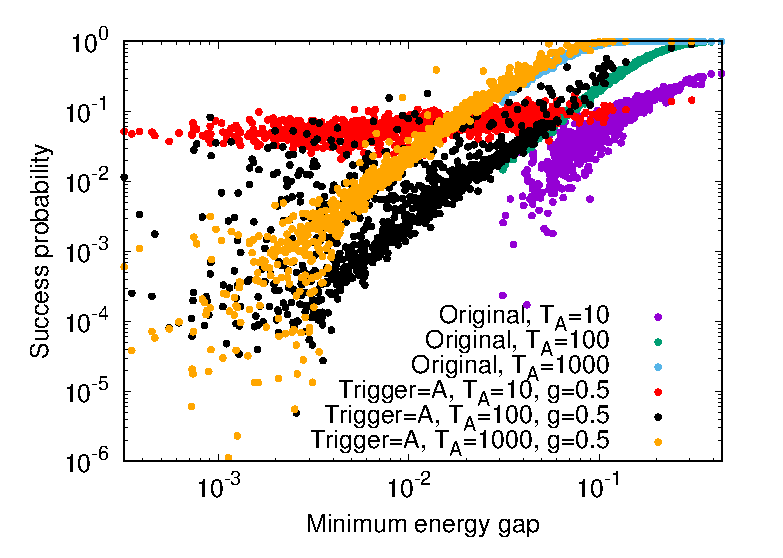
\includegraphics[scale=0.8]{SuccVsGap_OA_g0.eps}
\caption{Success probability versus minimum energy plot for all the problems belonging to the set of 12-spin SAT problems, for annealing times 10, 100 an 1000, in the absence and presence of the  antiferromagnetic trigger.}
\label{fig:a17}
\end{figure}


It can be noted from Fig.~(\ref{fig:a17}) that the original success probabilities mostly follow the Landau-Zener dependence on minimum energy gaps (\ref{eq:lz5}), although the scattering for $T_A$=10 is comparatively large. As the annealing time is increased, the scattering becomes less prominent. However, upon adding the trigger, the scattering becomes even larger, so that the points corresponding to $T_A$=10 appear rather flat. Additionally, the problems with smaller minimum gaps have a higher success probability for $T_A$=10 than for $T_A$=100, due to non-adiabatic evolution of the system in these problems. In this case too the curves become successively less scattered on increasing the annealing time and the general effect of adding the trigger with strength $g$=0.5 is to shift the points leftwards by reducing the minimum energy gaps.
\newpage

\section{Trigger strength g=1}
This section features the same analysis as the last section but with the value of the strength parameter $g$=1.\\
We begin by showing the distribution of the relative success probability after adding the antiferromagnetic trigger with $g$=1, for annealing times 10, 100 and 1000, in Fig.~(\ref{fig:a18}).
\begin{figure}
\centering 
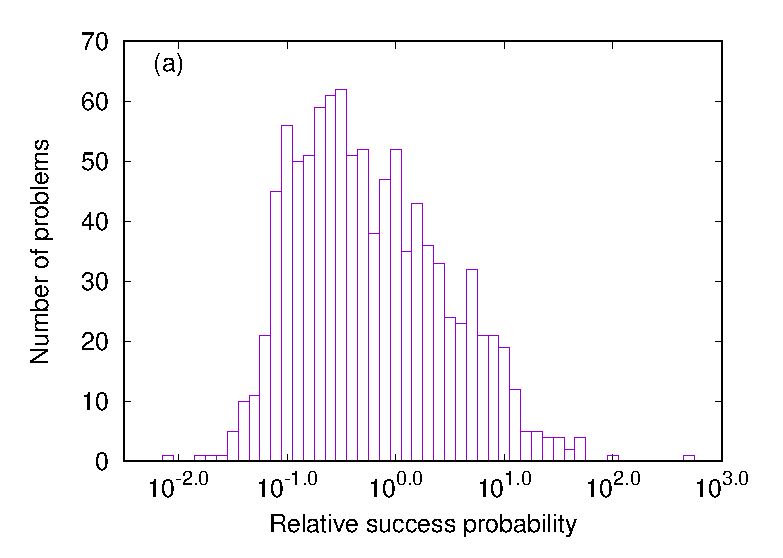
\includegraphics[scale=0.8]{A_T10_g1.eps}
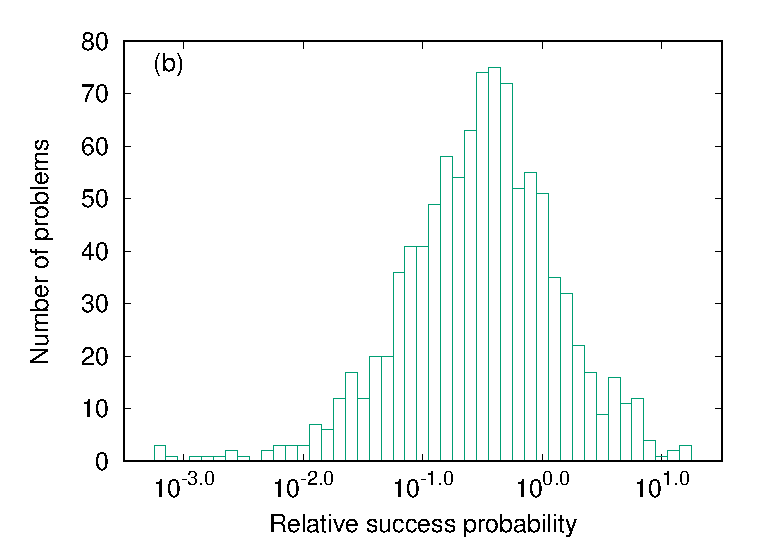
\includegraphics[scale=0.8]{A_T100_g1.eps}
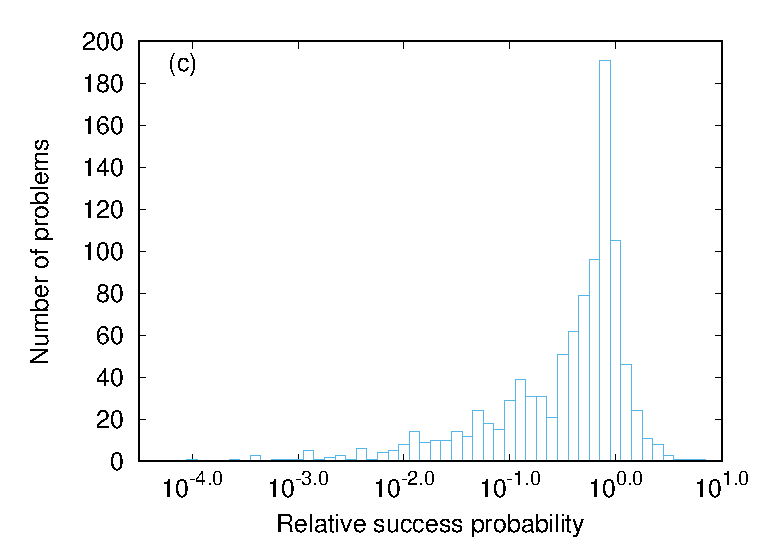
\includegraphics[scale=0.8]{A_T1000_g1.eps}
\caption{Distribution of the relative success probability $p^A/p^O$ for $g$=1. (a): $T_A$=10; (b): $T_A$=100; (c): $T_A$=1000.}
\label{fig:a18}
\end{figure}


We find that 377 problems have an improved success probability after adding the antiferromagnetic trigger for $T_A$=10. This number reduces to 215 and 200 upon increasing the annealing time to 100 and 1000 respectively. Moreover, as the annealing time is increased, the largest value of the relative success probability drops from 501 at $T_A$=10, to 15.85 at $T_A$=100, to 6.31 at $T_A$=1000. Again, to obtain more insight about the effects of adding the antiferromagnetic trigger with $g$=1, the minimum energy gaps are computed for all the problems of the set after adding the trigger. Figure~(\ref{fig:a21}) shows the resulting scatter plot between the minimum energy gaps after adding the antiferromagnetic trigger against the original minimum energy gaps.

\begin{figure}
\centering 
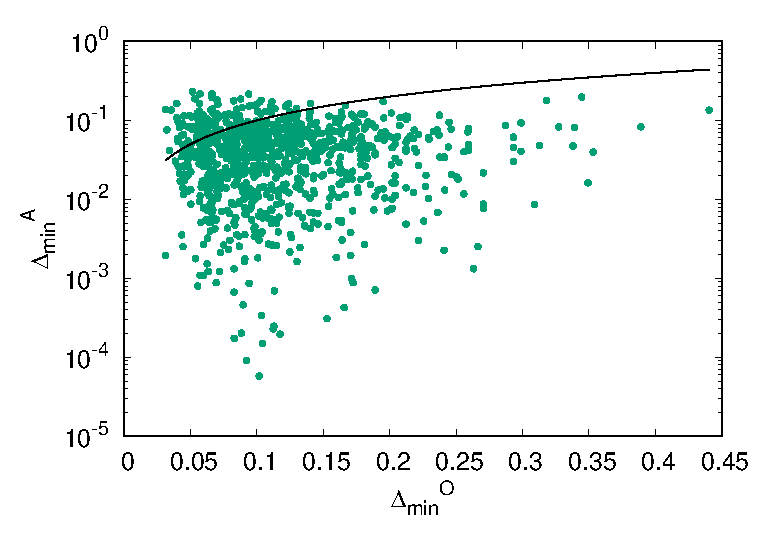
\includegraphics[scale=0.8]{MinGap_A_g1.eps}
\caption{A plot of the minimum energy gaps after adding the antiferromagnetic trigger with $g$=1 ($\Delta_{min}^A$), with the original minimum energy gaps ($\Delta_{min}^O$). For 879 problems the minimum energy gap decreases after adding the trigger.}
\label{fig:a21}
\end{figure}
In this case, 879 problems have smaller minimum energy gaps upon the addition of the trigger. Thus, a decrease in the success probability for most of the cases compared to the original, for all annealing times, seems to be plausible.

Furthermore, for most of the cases the number of energy anti-crossings between the ground state and the first excited state increases to 2, while in one case it was noted to be 4. Table~(\ref{tab:a4}) shows the number of cases with different number of anti-crossings.

\begin{table}[H]
\centering
\renewcommand{\arraystretch}{1.5}
\begin{tabular}{|c|c|}
\hline 
Number of anti-crossings & Number of cases  \\ 
\hline 
1 & 202 \\ 
\hline 
2 & 705 \\ 
\hline 
3 & 92 \\ 
\hline 
4 & 1 \\ 
\hline 
\end{tabular} 
\caption{Number of cases with different number of anti-crossings after adding the antiferromagnetic trigger.}
\label{tab:a4}

\end{table}
To obtain a feeling of the difficulty of the problems which have a relative success ratio greater than one, a scatter plot of the success probabilities after adding the antiferromagnetic trigger against the original success probabilities is shown in Fig.~(\ref{fig:a22}).


\begin{figure}
\centering 
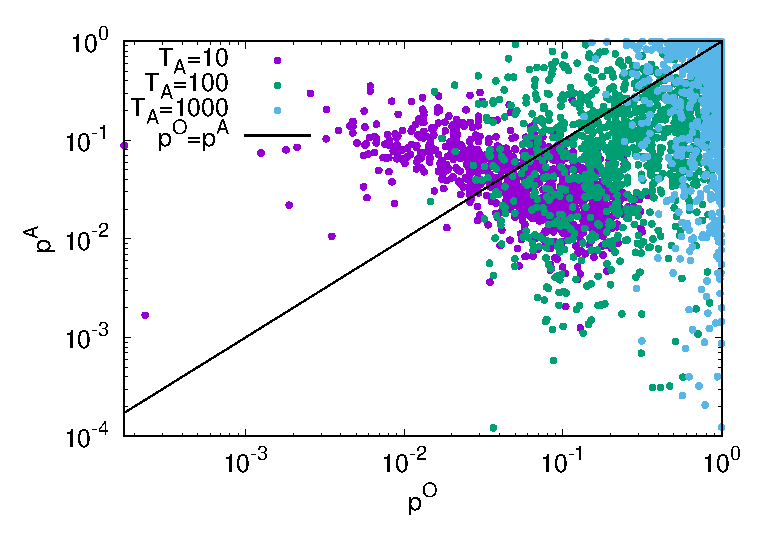
\includegraphics[scale=0.8]{ProbScat_g1.eps}
\caption{A plot of the success probabilities after adding the antiferromagnetic trigger with $g$=1 ($p^A$), with the original success probabilities ($p^O$) for annealing time 10, 100 and 1000.}
\label{fig:a22}
\end{figure}

Again, it can be noted that for $T_A$=10, the 377 problems that have a higher success probability after adding the antiferromagnetic trigger are limited to the cases with smaller original success probability (smaller minimum gaps). Since adding the trigger reduces the minimum energy gap in most of the cases, the cases with smaller $p^O$ mostly benefit from a non-adiabatic evolution (shorter annealing time).\\

To understand the role that the annealing time plays in improving the success probability, the scatter plots for the minimum energy gaps were plotted only for the problems with a relative success probability greater than 1 for a fixed annealing time. Figure~(\ref{fig:a23}) shows the resulting plots for annealing times of 10, 100 and 1000.\\

\begin{figure}
\centering 
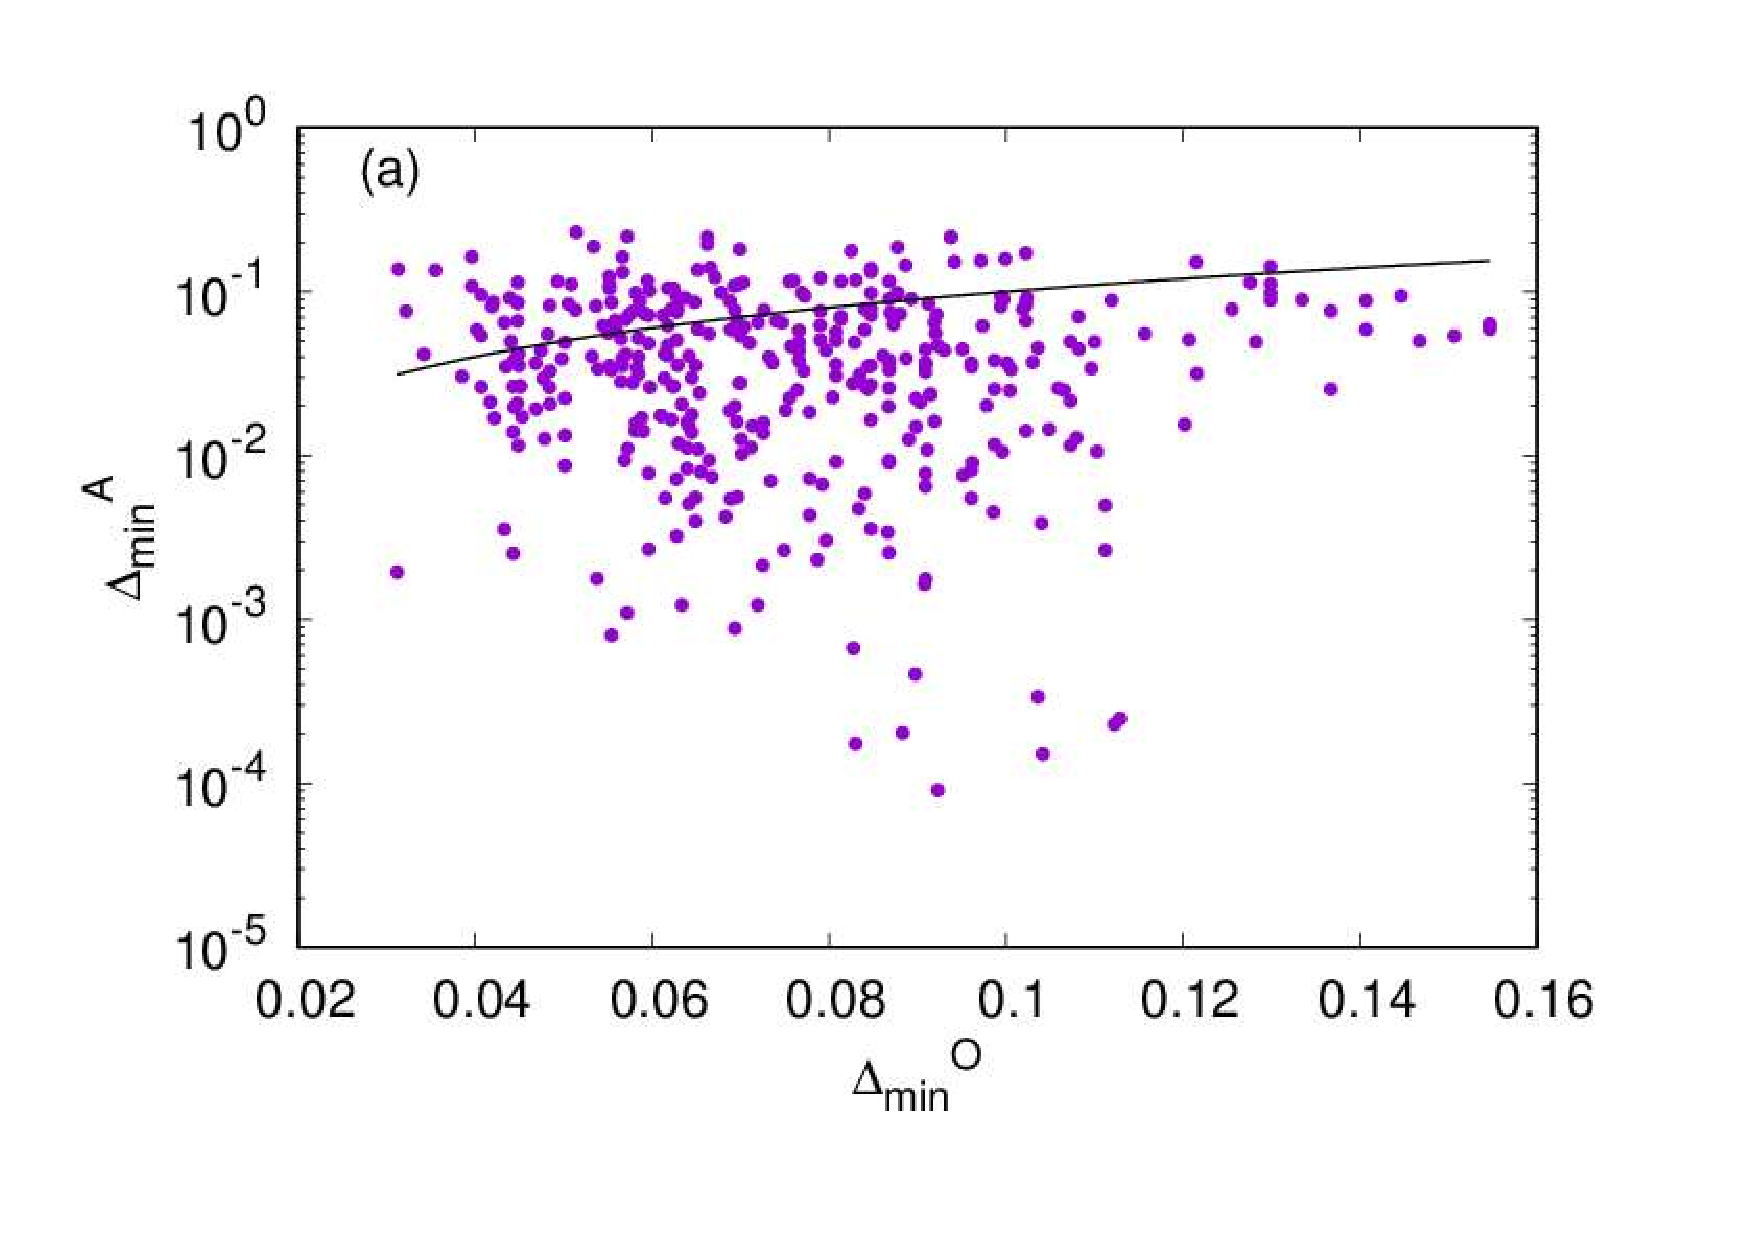
\includegraphics[scale=0.35]{selected_T10_g1.pdf}
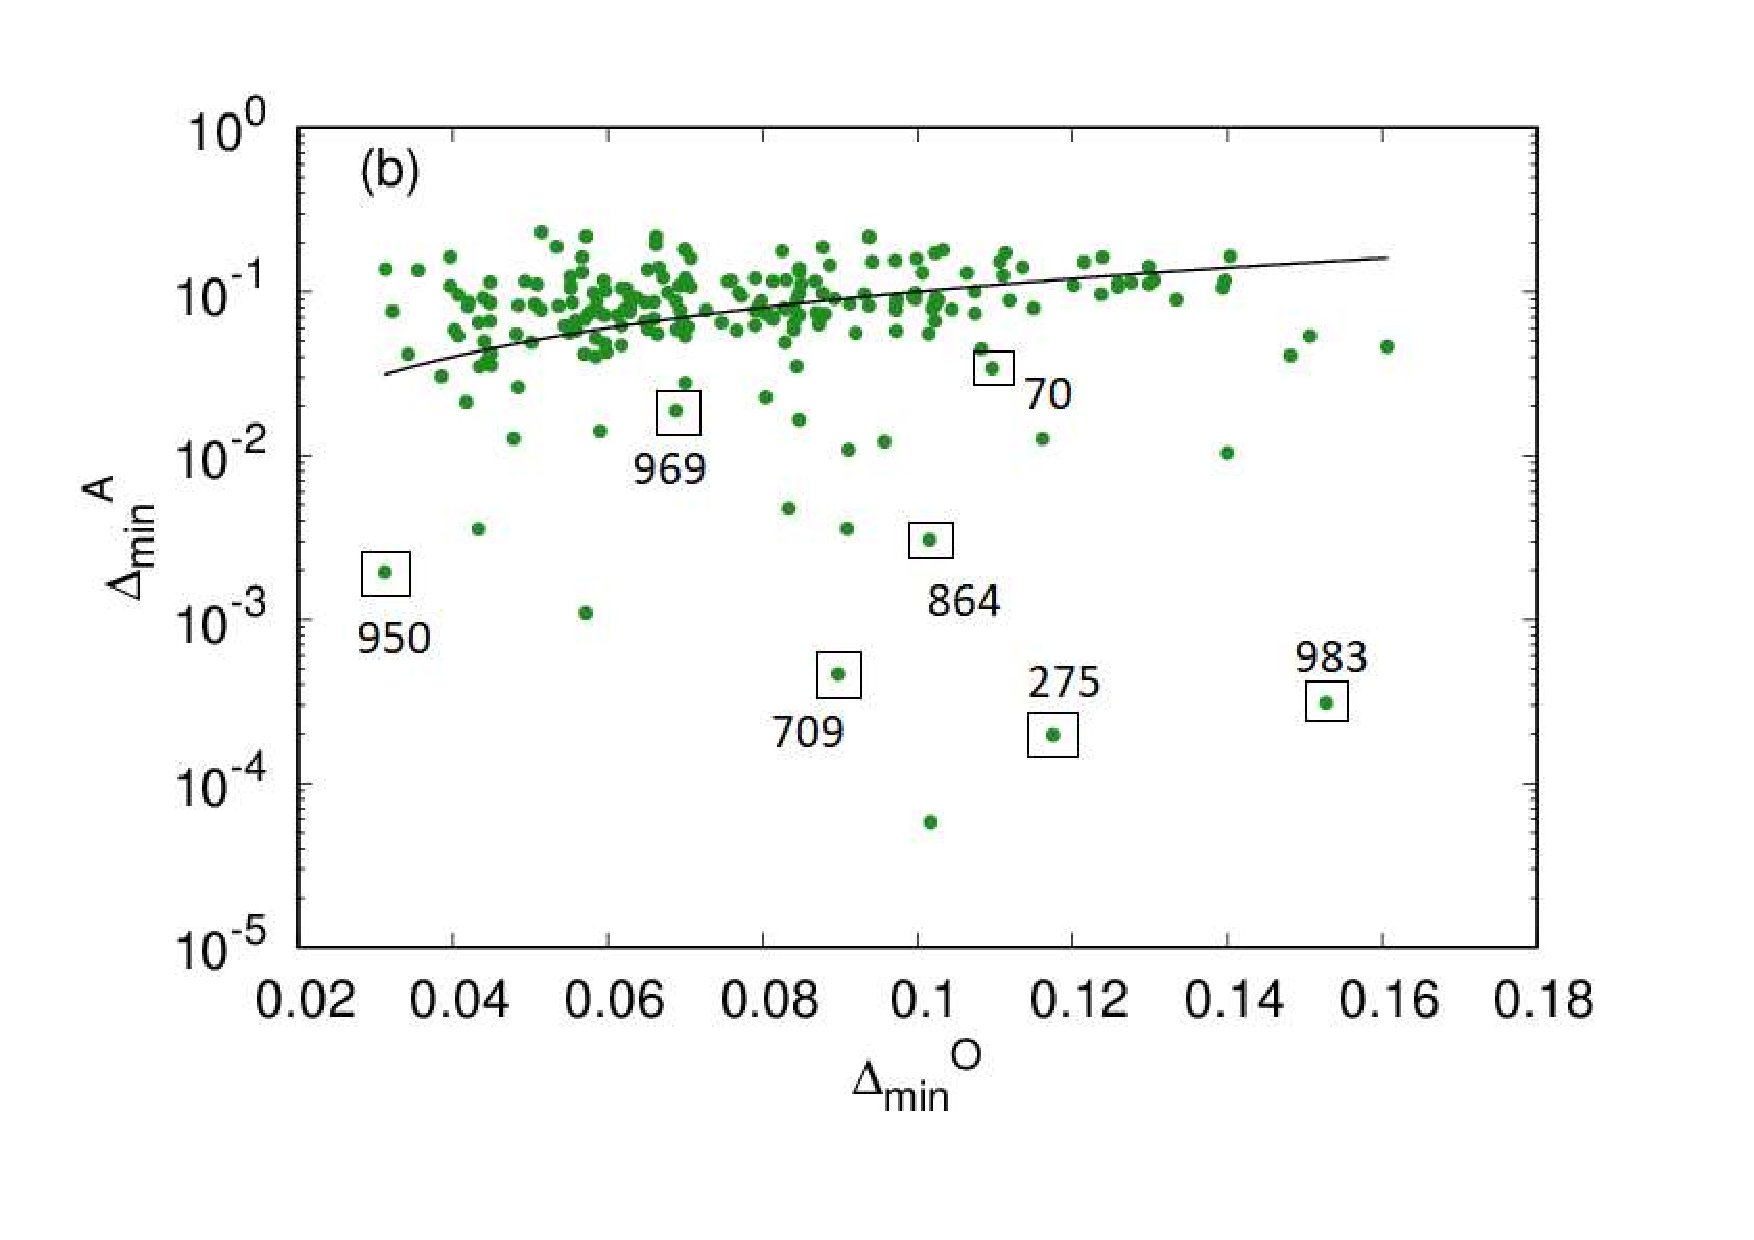
\includegraphics[scale=0.35]{selected_T100_g1.pdf}
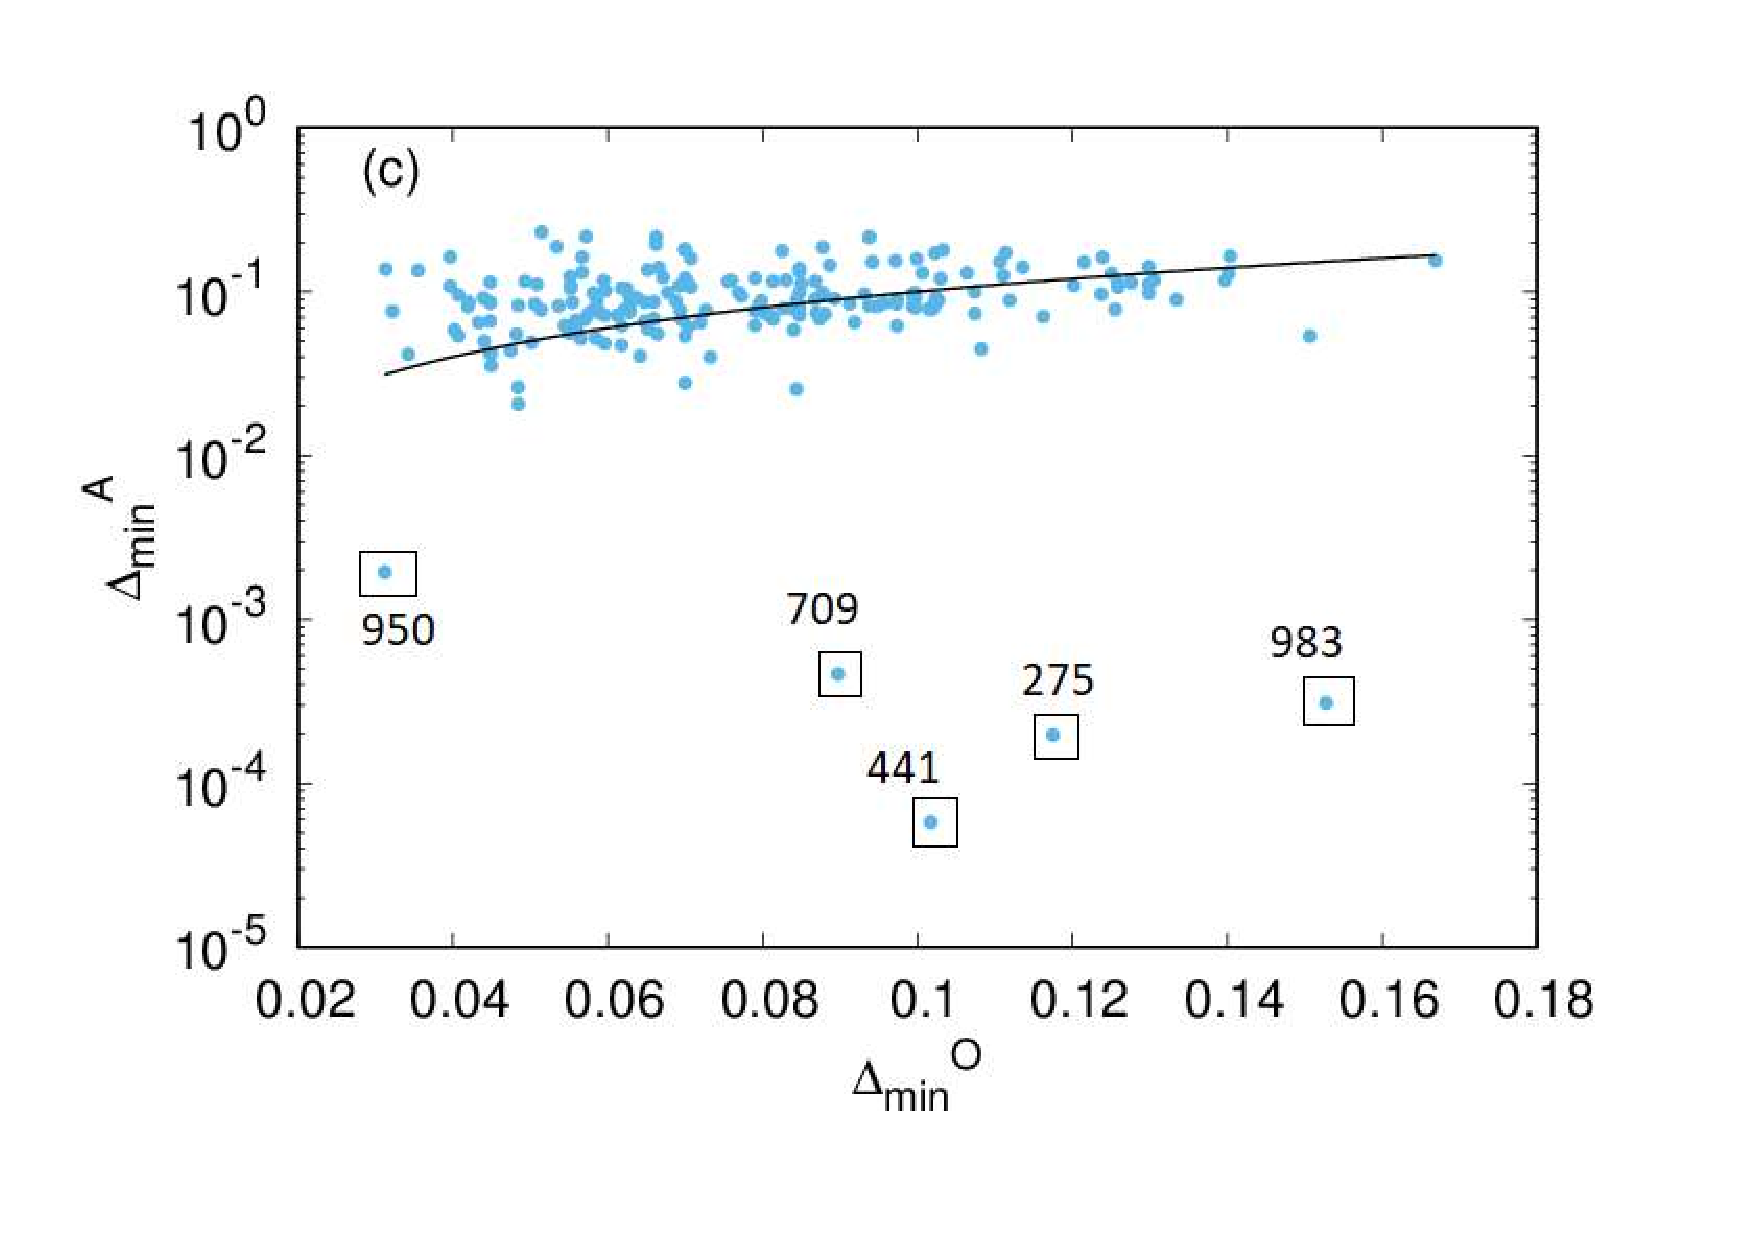
\includegraphics[scale=0.35]{selected_T1000_g1.pdf}
\caption{Scatter plot of energy gaps $\Delta^A $ with $\Delta^O$ for cases with improved success probability after adding the antiferromagnetic trigger with $g$=1. (a): $T_A=10$; (b): $T_A=100$; (c): $T_A=1000$. For a certain subset of the problems, the corresponding problem number is indicated next to the points.}
\label{fig:a23}
\end{figure}
Out of the 377 problems with higher success probability after adding the antiferromagnetic trigger for $T_A$=10, 279 problems have a reduced minimum energy gap as a consequence of adding the trigger. These problems can therefore be expected to be benefiting from a non-adiabatic evolution for small annealing time of $T_A$=10. On the other hand, for the rest 98 problems, the minimum gaps increase. It was noted that except for 2 cases (problems 325 and 705), all the problems with enlarged minimum gap and improved success probability for $T_A$=10 also have an improved success probability for $T_A$=100 and $T_A$=1000. This suggests that for these cases, adding the antiferromagnetic trigger increases the minimum energy gap enough to make the evolution closer to adiabatic even for $T_A$=10. 
\newpage

Additionally, for problems 325 and 705, the relative success probability is greater than 1 for $T_A$=10 and $T_A$=1000, while it is smaller than 1 for $T_A$=100. The energy spectra and the mechanism leading to this trend are similar for both these problems. Therefore, Fig.~(\ref{fig:a24}) shows the energy spectrum and the energy expectation values for the state, before and after adding the trigger for problem 705.

\begin{figure}[H]
\centering 
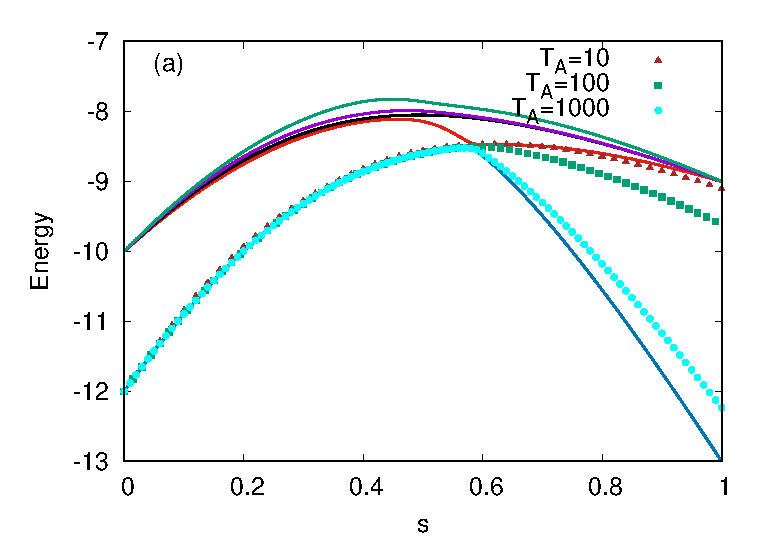
\includegraphics[scale=0.8]{705_O_T.eps}
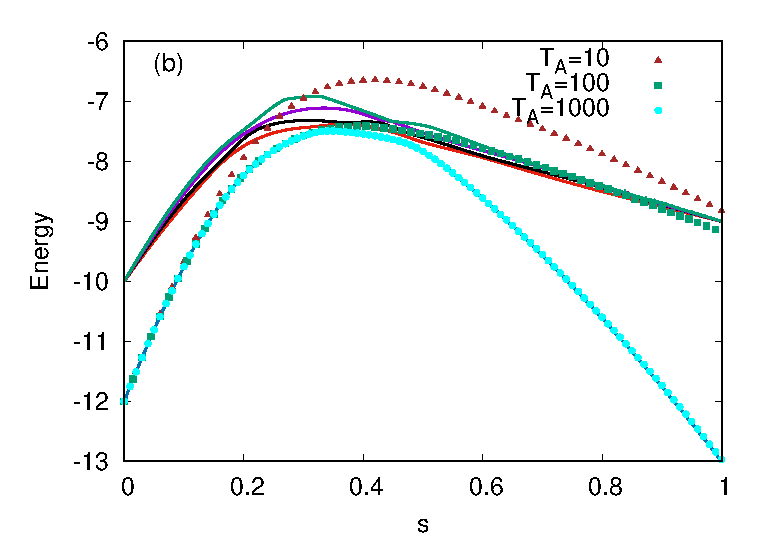
\includegraphics[scale=0.8]{705_A_T_g1.eps}
\caption{Energy spectrum and energy expectation values for the instantaneous state for problem 705. (a): Original Hamiltonian; (b): Antiferromagnetic Hamiltonian. }
\label{fig:a24}
\end{figure}

Although adding the trigger enlarges the minimum gap in these cases, the spectrum of the problem changes in a way such that the first excited state is present in the vicinity of the ground state for a longer time. In this particular case, this gives the system state a chance to transit to the higher energy levels even before the first energy anti-crossing for $T_A$=10, and end in a state with a larger overlap with the ground state than in the original case, where it closely follows the first excited state after the anti-crossing. For $T_A$=100, and in the presence of the trigger, the state shifts to the higher excited state at the second energy anti-crossing, but this time the overlap of the final state with the ground state is smaller than that in the case of the original Hamiltonian. Finally, an annealing time of $T_A$=1000 becomes long enough for the evolution to become adiabatic, and since the minimum energy gap is increased after adding the trigger, the success probability in the presence of the trigger becomes larger.\\

Next, from Fig.~(\ref{fig:a23}(b) and \ref{fig:a23}(c)) it can be noted that the majority of the problems improved by adding the antiferromagnetic trigger, and choosing the annealing time to be $T_A$=100 or $T_A$=1000 correspond to the cases where the minimum energy gaps become larger upon adding the trigger. Out of the 215 (200) problems improved after adding the trigger for $T_A$=100 ($T_A$=1000), 117 (121) problems have larger minimum gaps after including the trigger.\\
Some of the problems with an improved success probability despite of a reduced minimum energy gap were selected and their dynamics was studied. These have been marked in the middle and bottom panel of Fig.~(\ref{fig:a23}). 

It can be noticed that problems 275, 441, 709, 950 and 983 appear in both the figures. The conclusions drawn are the following:
\begin{itemize}
\item For problems 70, 275, 441, 709 and 864 the presence of two anti-crossings increases the overlap of the final state with the ground state of the Hamiltonian. Figure~(\ref{fig:a28}) shows the energy spectrum and the energy expectation values for the corresponding state for the original Hamiltonian, and the Hamiltonian after adding the antiferromagnetic trigger.


\begin{figure}
\centering 
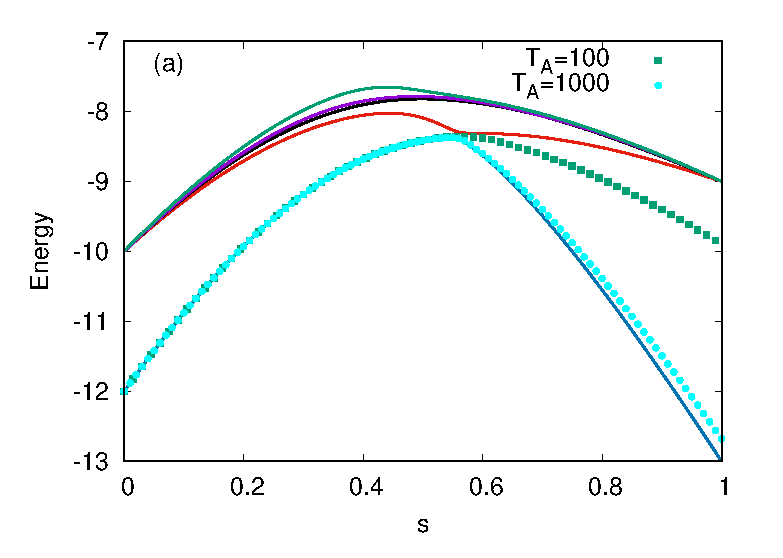
\includegraphics[scale=0.8]{441_O_T.eps}
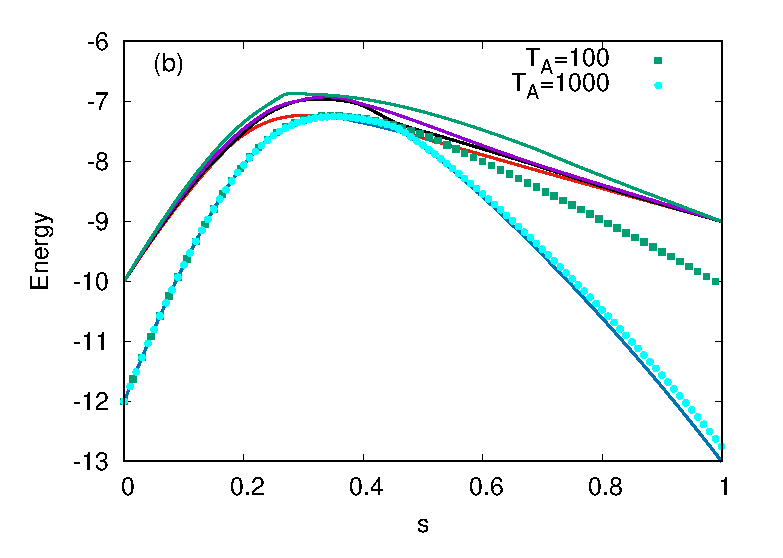
\includegraphics[scale=0.8]{441_A_g1_T100_1000.eps}
\caption{Energy spectrum and energy expectation values for the instantaneous state for problem 441. (a): Original Hamiltonian; (b) Antiferromagnetic Hamiltonian.}
\label{fig:a28}
\end{figure}


After adding the trigger to this problem, for both $T_A$=100 and $T_A$=1000, the system state shifts most of its amplitude to the first excited state at the first anti-crossing. On reaching the second anti-crossing, some of the amplitude of the state comes back to the ground state, thus increasing the success probability in these cases.

\item To understand the reasons for an improved success probability in problem 950, the overlap of the state of the system was computed with the three lowest energy states of the instantaneous Hamiltonian, for $T_A$=100. 

\begin{figure}
\centering
  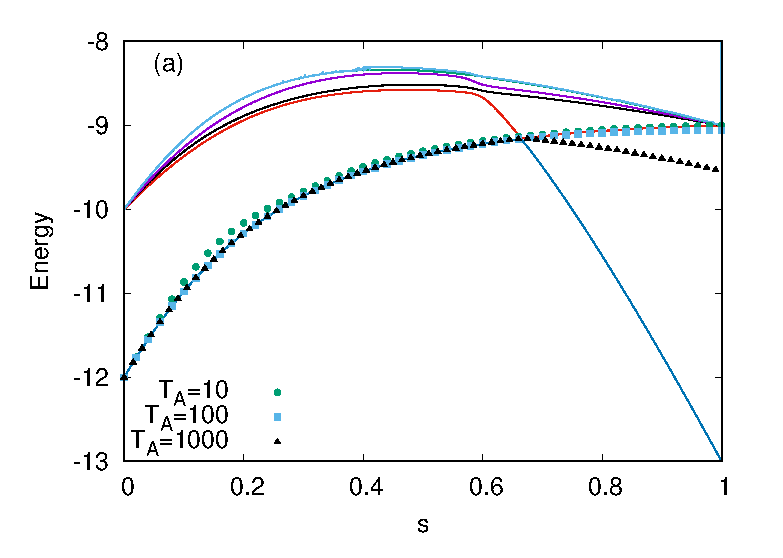
\includegraphics[scale=0.8]{950a_s12_O.eps}
  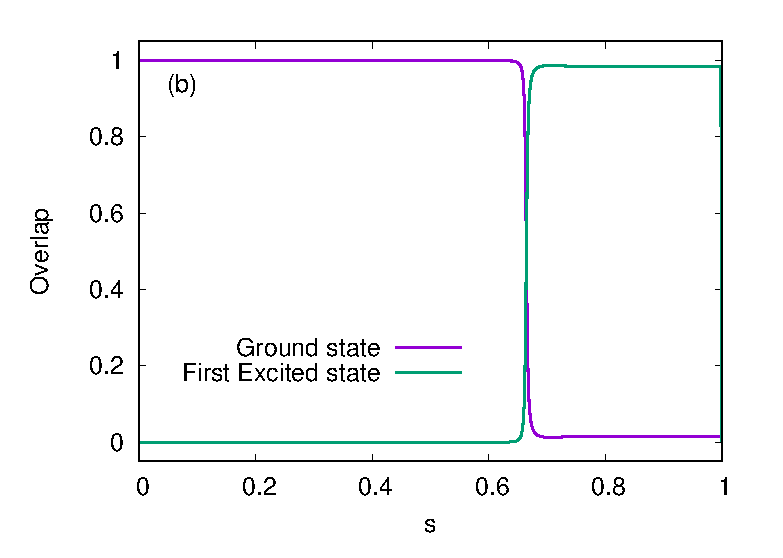
\includegraphics[scale=0.8]{950_Overlap_Orig.eps}
  \caption{Original Hamiltonian in Problem 950. (a): The energy spectra and instantaneous energy expectation values corresponding to $T_A$=100, and $T_A$=1000; (b): The overlap of the system state with the three lowest lying energy levels of the instantaneous Hamiltonian for $T_A$=100.}
  \label{fig:a30}
 \end{figure}
 
As can be observed on comparing Figs.~(\ref{fig:a30}(a)) and (\ref{fig:a32}(a)), the energy spectrum of problem 950 changes significantly upon adding the antiferromagnetic trigger. The minimum energy gap becomes smaller, and the two lowest energy states remain in close vicinity for longer. Unlike the shift of the state of the system to the first excited state at the anti-crossing, and following it closely thereafter in the original Hamiltonian for $T_A$=100 (see Fig.~(\ref{fig:a30}(b))), the dynamics of the state becomes more complex after including the antiferromagnetic trigger. It can be noted from Fig.~(\ref{fig:a32}(b)) that upon adding the trigger the system transits to the first excited state before the second anti-crossing, from where it shifts most of its amplitude to the second excited state. The remaining amplitude in the first excited state comes back to the ground state at the second anti-crossing, improving the success probability. Similar dynamics can be expected to benefit the case for $T_A$=1000 case as well.
\begin{figure}
\centering
  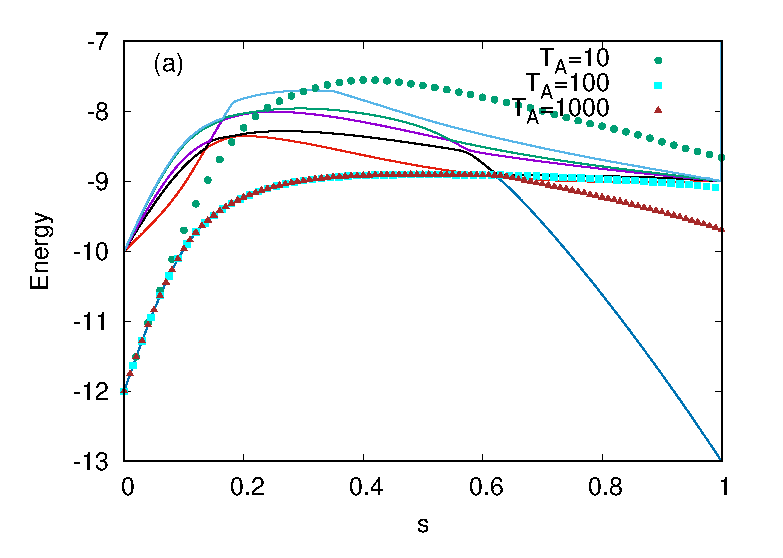
\includegraphics[scale=0.8]{950a_s12_A_g1.eps}
  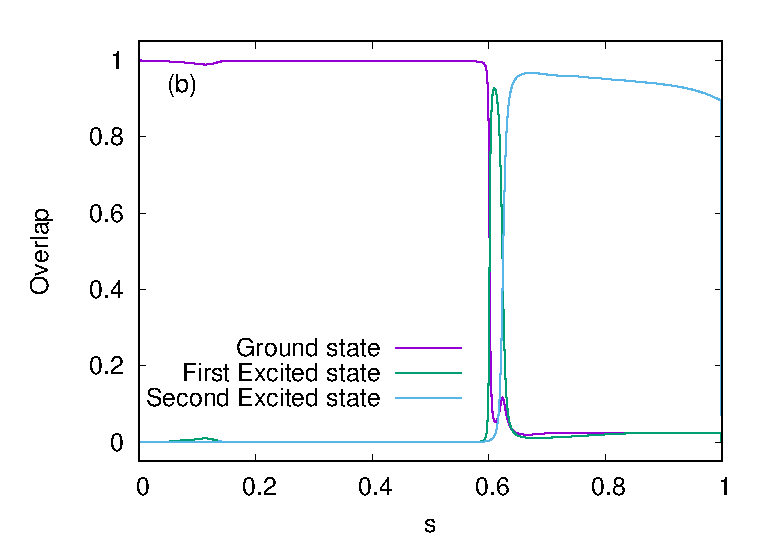
\includegraphics[scale=0.8]{950_A_g1_Overlap.eps}
  \caption{After adding antiferromagnetic Hamiltonian to Problem 950. (a): The energy spectra and instantaneous energy expectation values corresponding to $T_A$=100, and $T_A$=1000; (b): The overlap of the system state with the three lowest lying energy levels of the instantaneous Hamiltonian for $T_A$=100.}
   \label{fig:a32}
 \end{figure}



\item Again, to understand the exact dynamics in case of problem 969, the overlap of the system state with the three lowest energy levels of the Hamiltonian was computed. As was the case in the original Hamiltonian of problem 950, from Fig.~(\ref{fig:a47}) it can be observed that the system state shifts most of its amplitude to the first excited state at the anti-crossing, after which it stays close to the first excited state for the rest of the course. This decreases the overlap with the ground state, thus explaining the small success probability.
\begin{figure}
\centering
  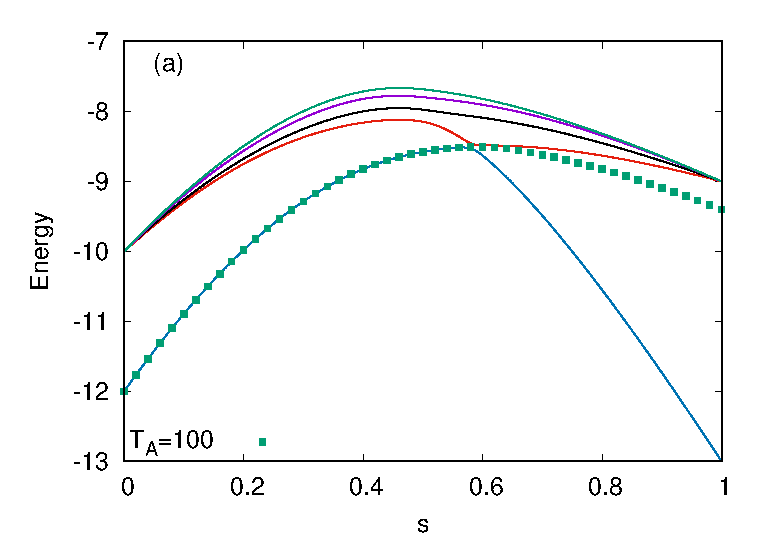
\includegraphics[scale=0.8]{969_O_T100.eps}
  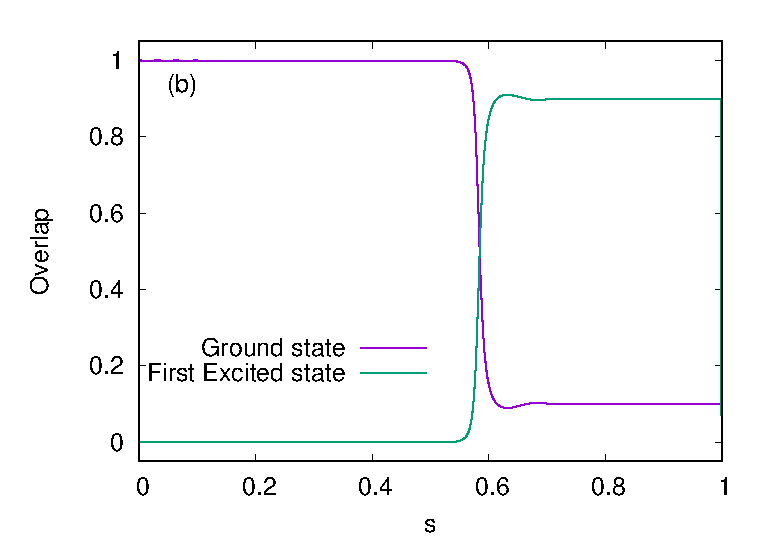
\includegraphics[scale=0.8]{969_Overlap_Orig.eps}
  \caption{Original Hamiltonian in Problem 969. (a): The energy spectra and instantaneous energy expectation values corresponding to $T_A$=100, and $T_A$=1000; (b): The overlap of the system state with the three lowest lying energy levels of the instantaneous Hamiltonian for $T_A$=100.}
    \label{fig:a47}
 \end{figure}

Figure~(\ref{fig:a49}(b)) makes it clear that on adding the antiferromagnetic trigger the system state shifts to the first excited state at the first anti-crossing. It shifts the amplitude further to the close lying higher excited states. However, since the first and second excited states stay close enough for a long time, so that the state continuously exchanges the amplitude between these states, the overlap with these states oscillates. As the state approaches the second anti-crossing, the amplitude present in the second excited state shifts back to ground state.
\begin{figure}
\centering
  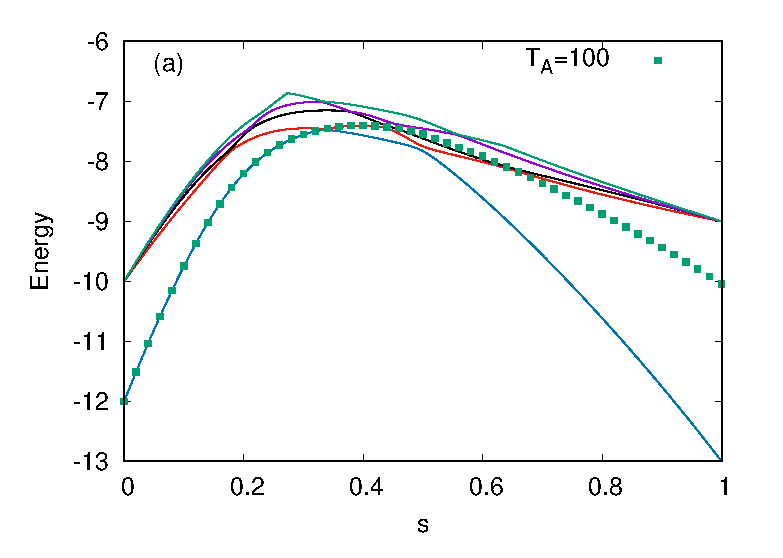
\includegraphics[scale=0.8]{969_A_T100_g1.eps}
  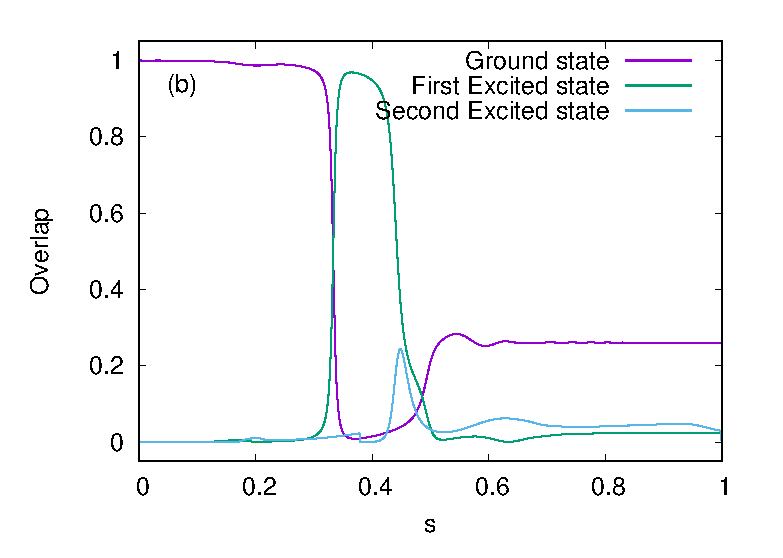
\includegraphics[scale=0.8]{969_A_g1_Overlap.eps}
  \caption{After adding antiferromagnetic Hamiltonian to Problem 969. (a): The energy spectra and instantaneous energy expectation values corresponding to $T_A$=100, and $T_A$=1000; (b): The overlap of the system state with the three lowest lying energy levels of the instantaneous Hamiltonian for $T_A$=100.}
  \label{fig:a49}
 \end{figure}

\item  Finally, for problem 983, Fig.~(\ref{fig:a51}) shows the energy gap between the lowest two energy levels as a function of the annealing parameter $s$, for the original Hamiltonian, and after adding the antiferromagnetic trigger. The minimum energy gap after adding the trigger becomes wider, so that the ground state and the first excited state stay close for longer. This gives the state a chance to redistribute the amplitude between these states. Therefore, despite the decrease in the minimum energy gap, there is a larger amplitude in the ground state in this case, compared to that in the original Hamiltonian.

\begin{figure}[H]
  \centering
  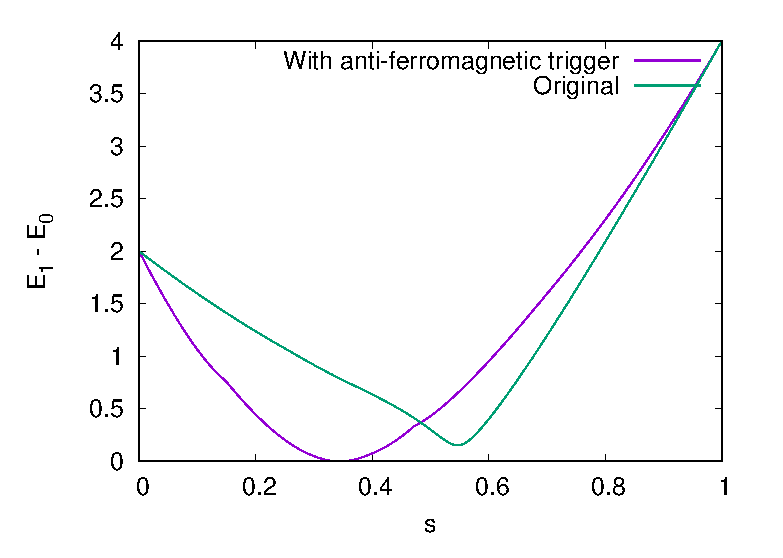
\includegraphics[scale=0.8]{983_Mingap.eps}

\caption{Energy gap between the ground state and the first excited state of the original Hamiltonian, and that after adding the antiferromagnetic trigger with $g$=1.}
  \label{fig:a51}
\end{figure}
\end{itemize}

Figure~(\ref{fig:a36}) shows the plot for the success probabilities for different problems against the corresponding minimum gaps.

\begin{figure}[H]
\centering 
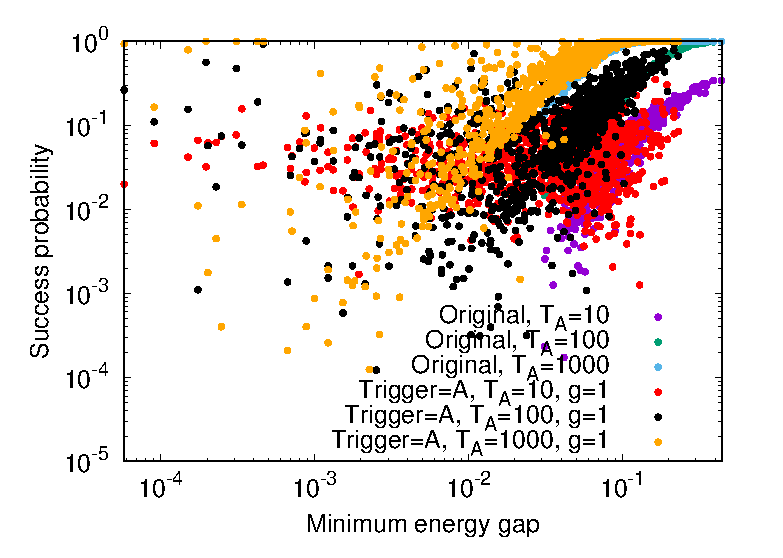
\includegraphics[scale=0.8 ]{SuccVsGap_OA_g1.eps}
\caption{Success probability versus minimum energy plot for all the problems belonging to the set of 12-spin problems, for annealing times 10, 100 and 1000, in the absence and presence of the antiferromagnetic trigger.}
\label{fig:a36}
\end{figure}

It can be seen that compared to the success probability versus minimum energy gap corresponding to the Hamiltonian where the antiferromagnetic trigger is added with $g$=0.5 (see Fig.~(\ref{fig:a17})), the scattering in case of adding the antiferromagnetic trigger with $g$=1 is larger for all the three annealing times. This indicates that the success probability is benefiting through non-adiabatic mechanisms for a larger fraction of problems in this case. One of the plausible reasons for this can be the increased number of energy anti-crossings between the ground state and the first excited state of the Hamiltonian. It can also be observed that unlike in Fig.~(\ref{fig:a17}), the curves for this case can be more easily distinguished to roughly have the Landau-Zener form, and that the points are not as restricted towards the left as a consequence of adding the trigger. This can be attributed to the presence of cases with enlarged minimum energy gaps as well.


\section{Trigger Strength g=2}
Finally, in this section the effects of adding the antiferromagnetic trigger with strength $g$=2 are discussed.\\
Figure~(\ref{fig:a37}) shows the distribution of the relative success probability after adding the antiferromagnetic trigger for $T_A$=10 and $T_A$=100. In this case, only 15 problems have an improved success probability after adding the trigger for $T_A$=10. Upon increasing the annealing time to 100, this number increases to 158, and to 225 for $T_A$=1000. This is in contrast with the observations from the previous sections where the number of the problems with improved success probability is maximal for $T_A$=10. 

\begin{figure}
\centering 
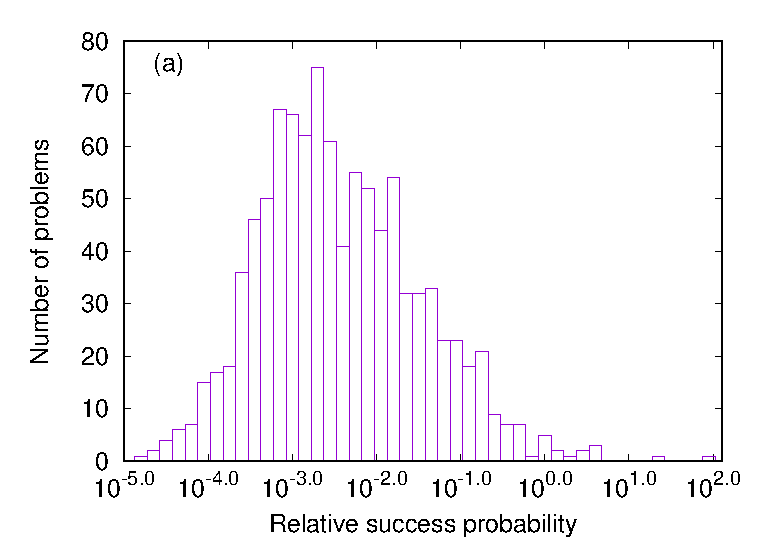
\includegraphics[scale=0.8 ]{A_T10_g2.eps}
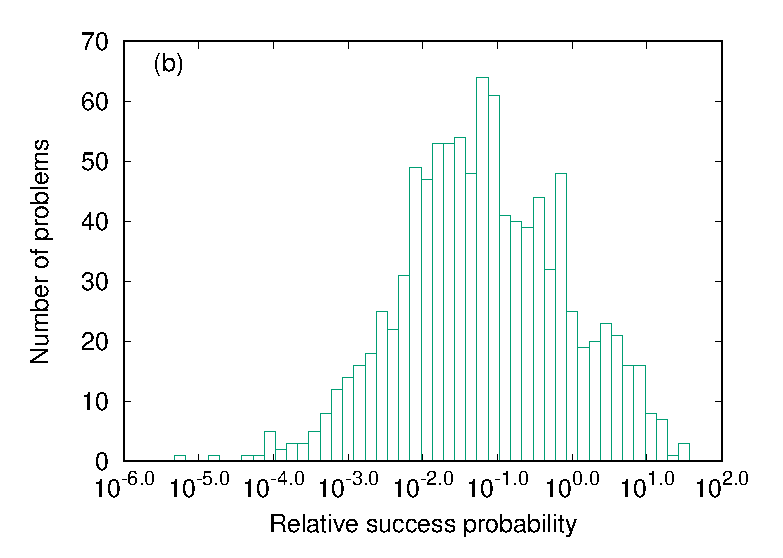
\includegraphics[scale=0.8 ]{A_T100_g2.eps}
\caption{Distribution of the relative success probability $p^A/p^O$ for $g$=0.5. (a): $T_A$=10; (b): $T_A$=100.}
\label{fig:a37}
\end{figure}
Furthermore, for $T_A$=1000 the spread of the relative success probability is only from 0.63 to 1.58, i.e. the effect of adding the trigger is only marginal. Additionally, for 448 problems the relative success probability is 1. For this reason the histogram for the distribution of the success probability for $T_A$=1000 is omitted.

Figure~(\ref{fig:a39}) shows the scatter plot of the minimum energy gaps after adding the antiferromagnetic trigger ($\Delta^A$) against the original minimum energy gaps ($\Delta^O$), for $g$=2. In this case, the minimum energy gaps reduce for 798 problems upon adding the trigger. It can also be noted that with the antiferromagnetic trigger of strength 2 the energy spectrum changes significantly in terms of the number of anti-crossings between the ground and the first energy level, and the proximity of the higher energy levels. Table~(\ref{tab:a5}) shows the number of cases with different number of anti-crossings.
\begin{table}[H]
\centering
\renewcommand{\arraystretch}{1.5}
\begin{tabular}{|c|c|}
\hline 
Number of anti-crossings & Number of cases \\ 
\hline 
1 & 1 \\ 
\hline 
2 & 132 \\ 
\hline 
3 & 439 \\ 
\hline 
4 & 33 \\ 
\hline 
5 & 65 \\
\hline
\end{tabular} 
\caption{Number of cases with different number of anti-crossings after adding the antiferromagnetic trigger with $g$=2.}
\label{tab:a5}

\end{table}
\begin{figure}
\centering 
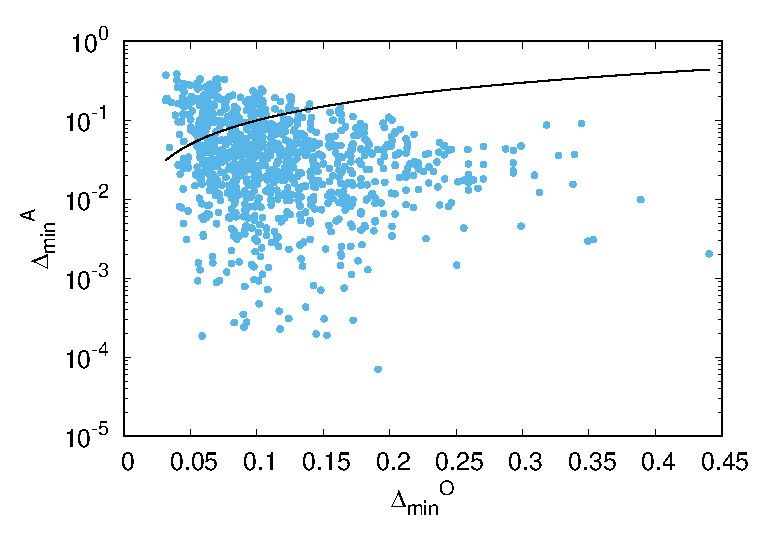
\includegraphics[scale=0.8 ]{MinGap_A_g2.eps}
\caption{A plot of the minimum energy gaps after adding the antiferromagnetic trigger with $g$=2 ($\Delta_{min}^A$), with the original minimum energy gaps ($\Delta_{min}^O$). For 798 problems the minimum energy gap decreases after adding the trigger.}
\label{fig:a39}
\end{figure}

Next, to assess the difficulty of problems affected by adding the antiferromagnetic trigger to the Hamiltonian, Fig.~(\ref{fig:a40}) shows the scatter plot of the success probabilities upon including the antiferromagnetic trigger ($p^A$) with the original success probabilities ($p^O$). 


\begin{figure}
\centering 
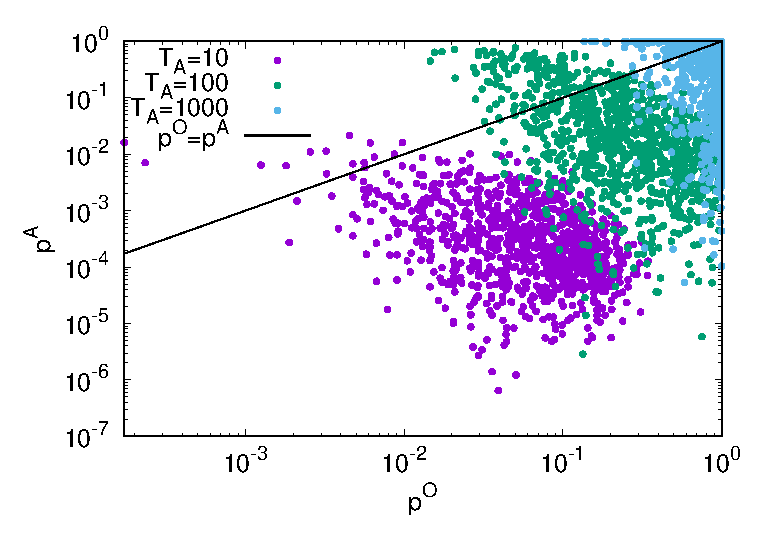
\includegraphics[scale=0.8]{ProbScat_g2.eps}
\caption{A plot of the success probabilities after adding the antiferromagnetic trigger with $g$=2 ($p^A$), with the original success probabilities($p^O$) for annealing time 10, 100 and 1000.}
\label{fig:a40}
\end{figure}
In this case too, the spread of the problems improved by adding the trigger is the largest for $T_A$=10. This can be attributed to the small original success probability ($p^O$) for a small annealing time of $T_A$=10, or to the non-adiabatic evolution mechanisms leading to a larger overlap with the ground state. In this case the problems with the three largest relative success probabilities corresponding to $T_A$=10, have smaller original success probabilities accounting for large improvements (the maximum relative success probability is 93.91). For $T_A$=100 and $T_A$=1000 the improvements become successively limited, with maximum relative success probabilities being 41.36 and 7.34 respectively. This is a consequence of increasing original success probabilities for longer annealing times. To understand the role that the annealing time plays in improving the success probability, the scatter plots for the minimum energy gaps are plotted only for the problems with a relative success probability greater than 1 for a fixed annealing time. Figure~(\ref{fig:a41}) shows the resulting plots for annealing times of 10, 100 and 1000.\\


\begin{figure}
\centering 
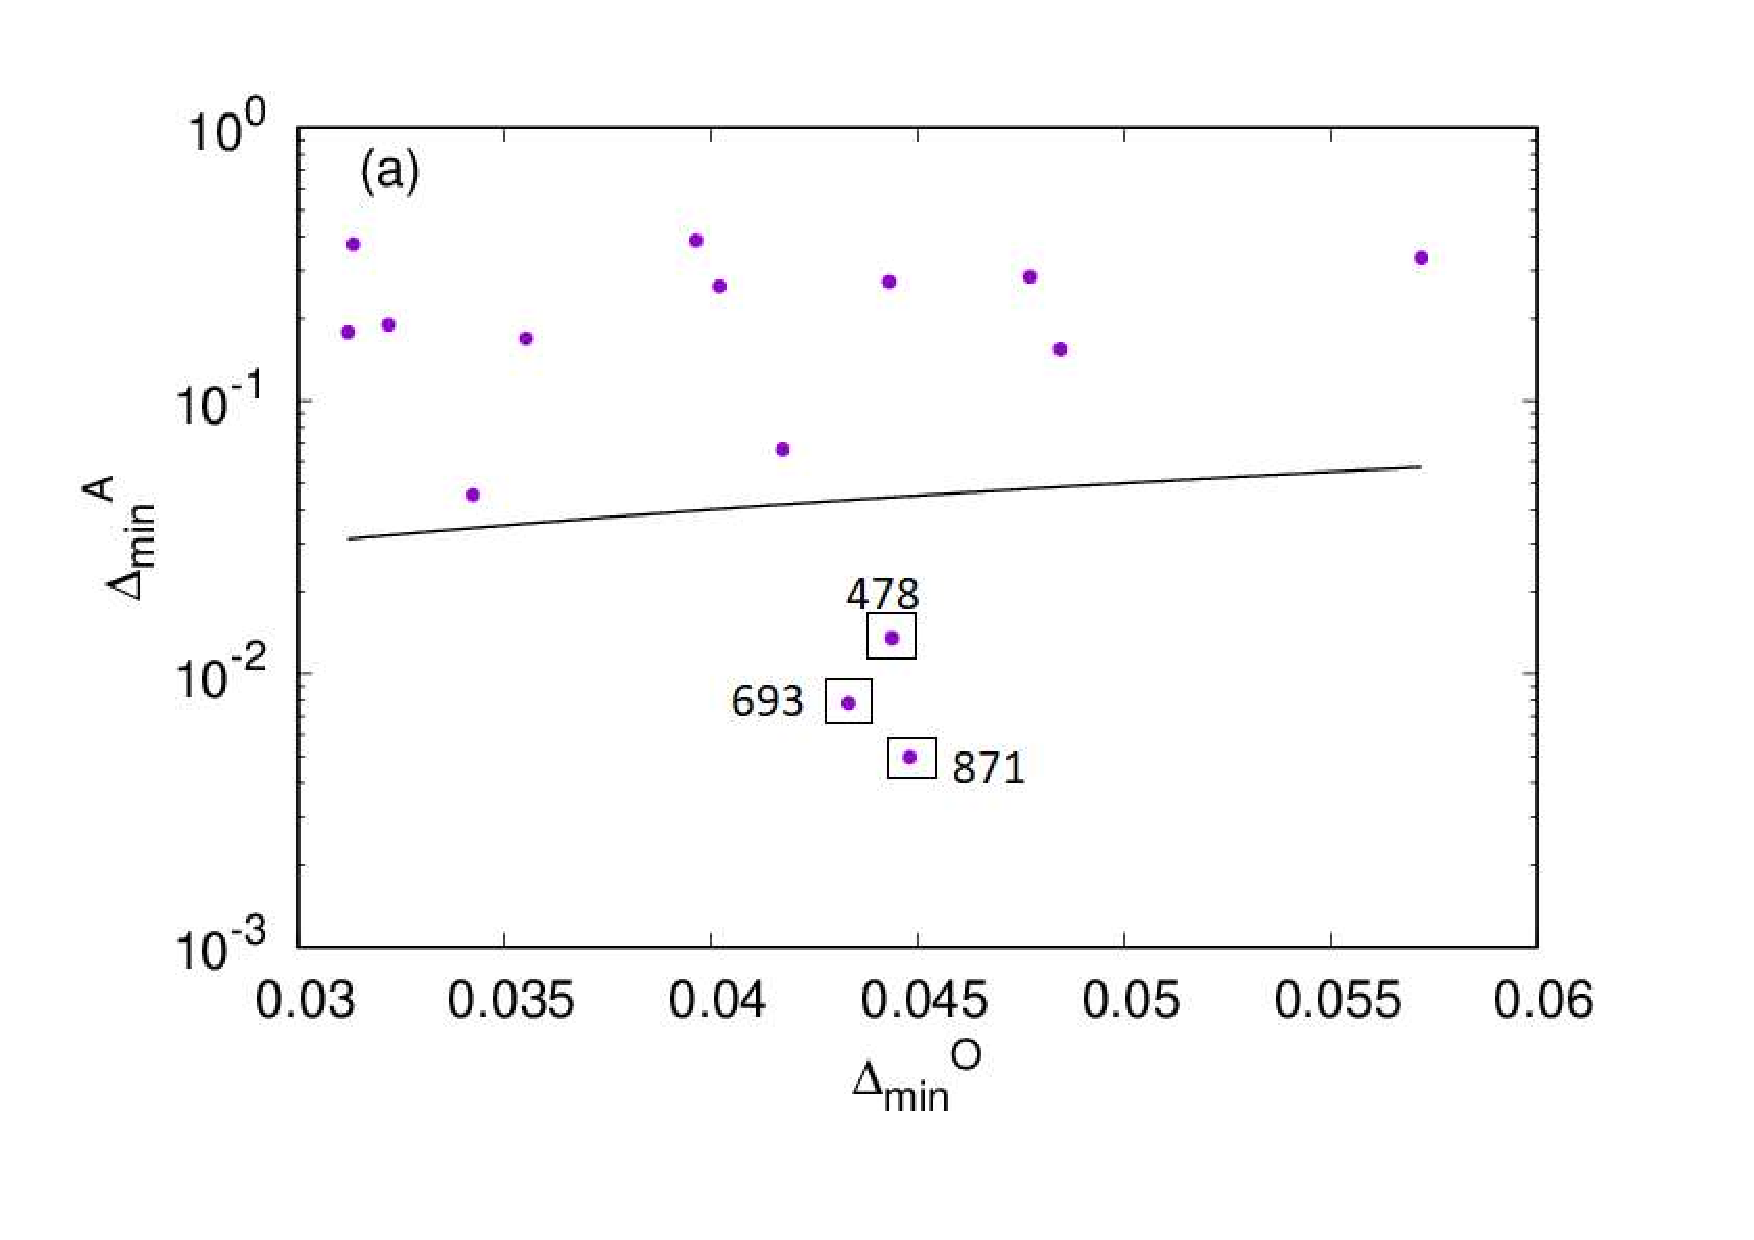
\includegraphics[scale=0.35 ]{selected_T10_g2.pdf}
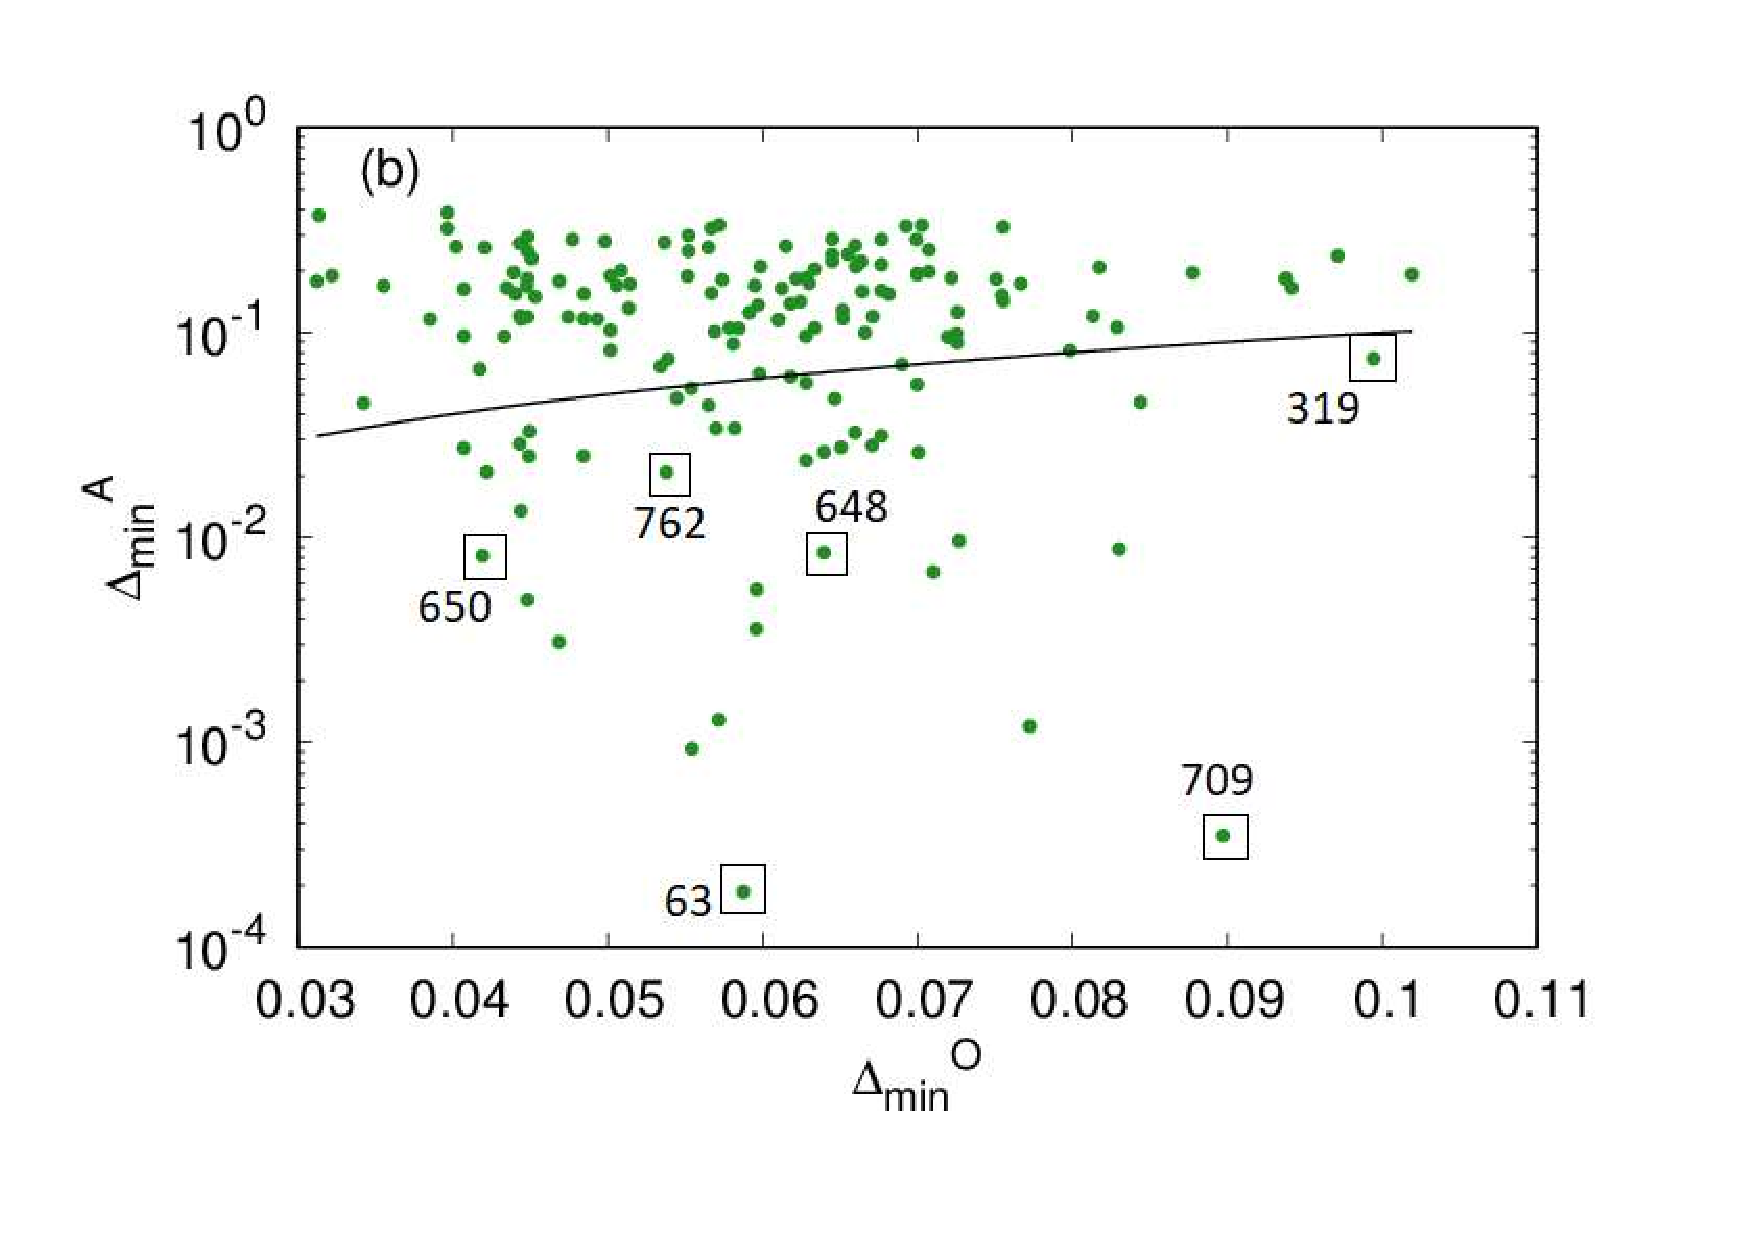
\includegraphics[scale=0.35 ]{selected_T100_g2.pdf}
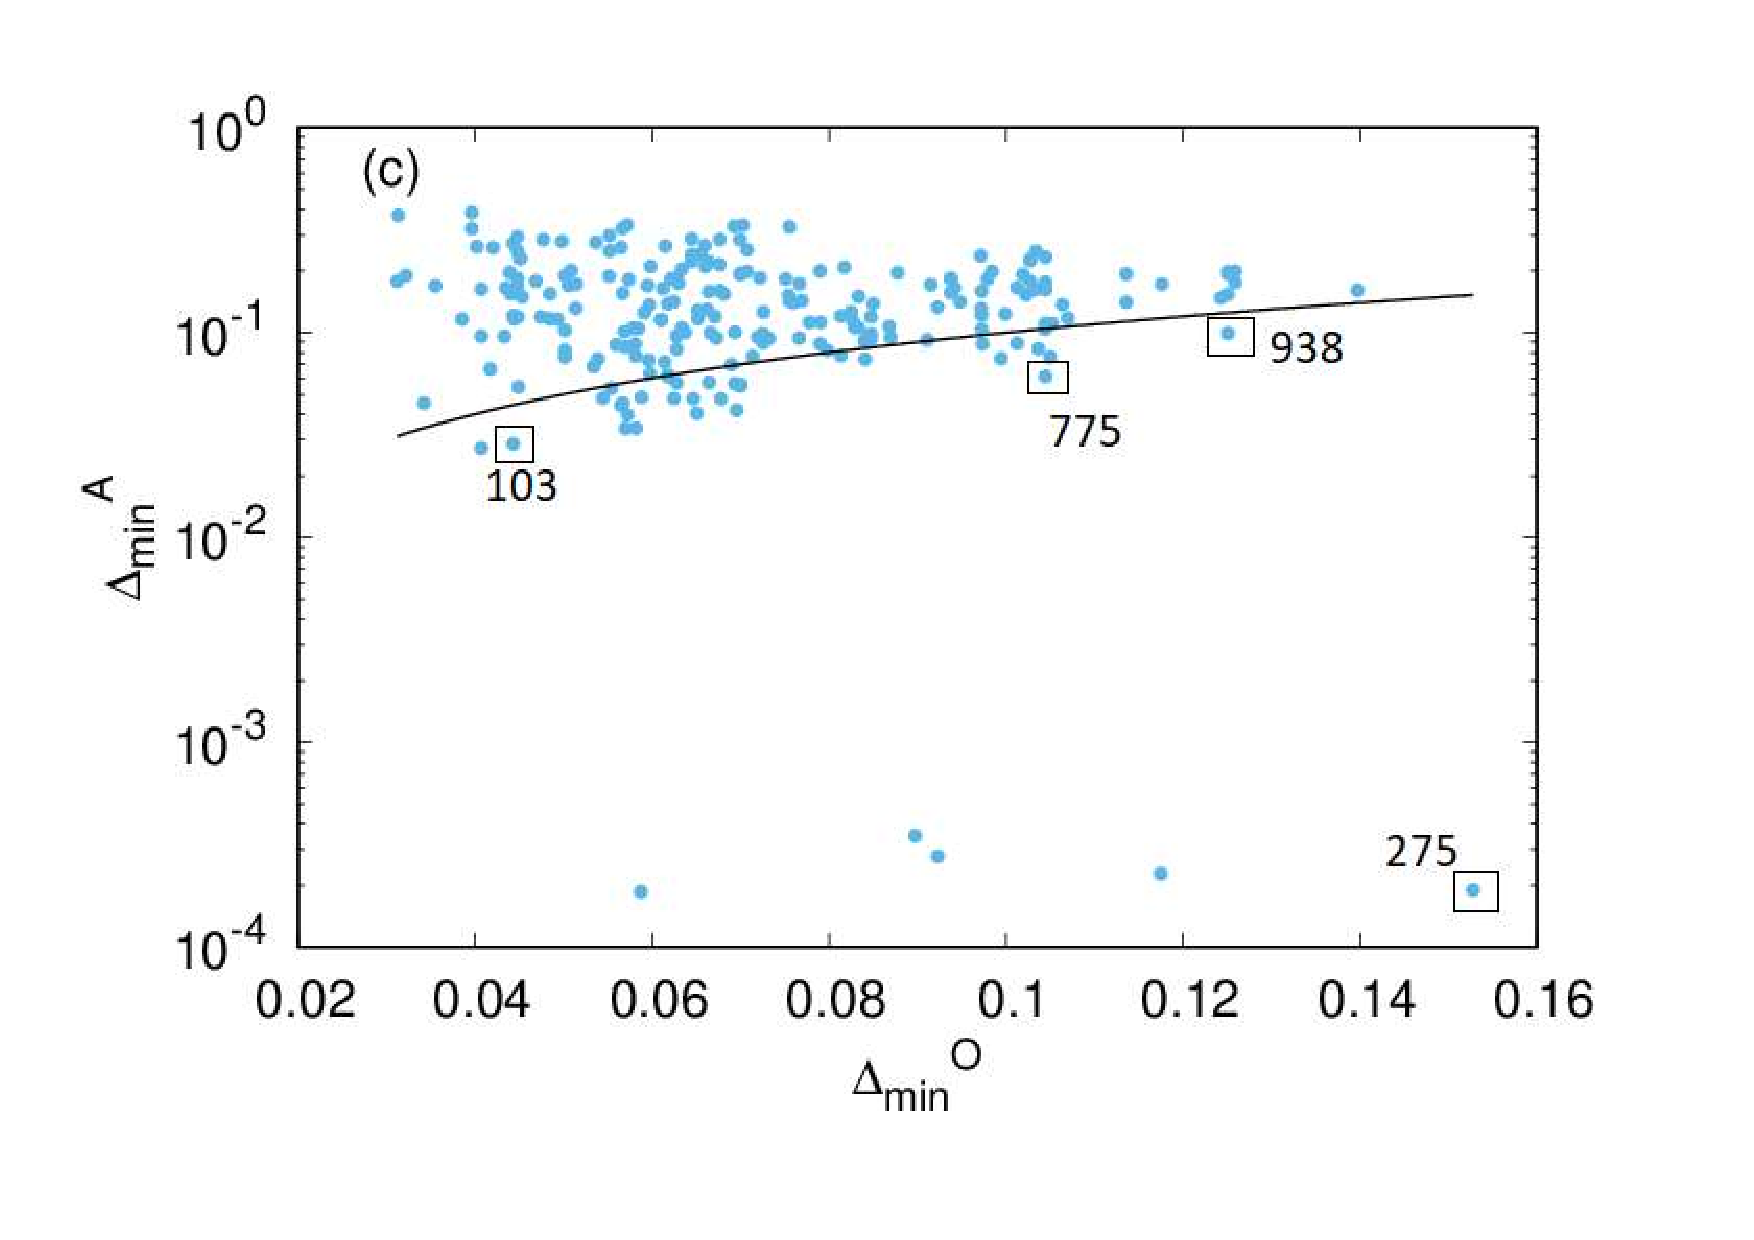
\includegraphics[scale=0.35 ]{selected_T1000_g2.pdf}
\caption{Scatter plot of energy gaps $\Delta^A $ with $\Delta^O$ for cases with improved success probability after adding the antiferromagnetic trigger with $g$=2. (a): $T_A=10$; (b): $T_A=100$; (c): $T_A=1000$.}
\label{fig:a41}
\end{figure}

From Fig.~(\ref{fig:a41}), it can be noted that 12 out of the 15 problems with an improved success probability for $T_A$=10, have larger minimum energy gaps upon including the antiferromagnetic trigger. It can be seen that all of these problems have an improved success probability for longer annealing times of 100 and 1000 as well. This suggests that adding the trigger widened the minimum energy gap enough for the evolution to become closer to adiabatic even for $T_A$=10.\\

However, unlike the case in the previous sections, only 3 problems (problem number 478, 693 and 871) with an improved success probability for $T_A$=10, have a smaller minimum energy gap after adding the antiferromagnetic trigger. All these problems are benefited from the similar non-adiabatic evolution of the state. The energy spectrum and the instantaneous energy expectation values of the state for the original Hamiltonian and the Hamiltonian after adding the trigger have been shown in Fig.~(\ref{fig:a42}) for problem 693. For the original Hamiltonian, the state of the system shifts to the first excited state on approaching the energy anti-crossing, and closely follows it thereafter. This makes the overlap of the system state with the ground state negligible. However, in the case where the antiferromagnetic trigger is included, the minimum energy gap reduces, making it feasible for the system to transit to the higher excited levels. Consequently, the system state ends in a superposition state consisting of higher energy levels, which has a larger overlap with the ground state of the Hamiltonian.


\begin{figure}
\centering 
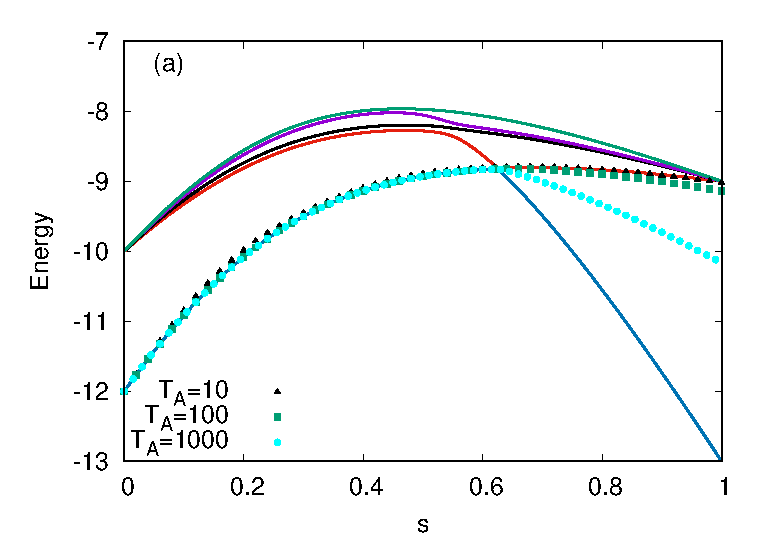
\includegraphics[scale=0.8]{693_O_g2.eps}
\includegraphics[scale=0.8]{693_A_g2.eps}
\caption{Problem 693: Energy spectrum and instantaneous energy expectation values.  (a): Original Hamiltonian; (b): Hamiltonian after adding the antiferromagnetic trigger.}
\label{fig:a42}
\end{figure}

In this problem, the success probability after adding the trigger reduces for both $T_A$=100 and $T_A$=1000. For the spectrum with the trigger and $T_A$=100, the system state shifts to the first excited state at the first anti-crossing, from where it soon shifts to the higher excited states. Unlike the case for $T_A$=10, this time the state follows them closely, resulting in a vanishing overlap with the ground state. For $T_A$=1000, on the other hand, the state shifts to the first excited state only on reaching the second anti-crossing. Since the original minimum gap is larger for this problem, the original success probability is larger for this annealing time.


Out of the 158 problems found to have an improved success probability after adding the trigger for $T_A$=100, 118 problems also have a larger minimum energy gap as a result of adding the trigger. It can be further noted that all of these cases have a relative success probability greater than 1 for $T_A$=1000 as well. The energy spectra for some of the remaining 40 cases were studied to understand the evolution of the state. Non-adiabatic mechanisms are responsible for the improvement in the success probabilities in all these cases.
For $T_A$=1000, 189 out of the 225 cases with an improved success probability upon including the antiferromagnetic trigger, have a larger minimum energy gap after adding the trigger. The energy spectra for some of the remaining 36 cases were also studied, of which 13 problems also to have a larger success probability for $T_A$=100.\\

A problem with an interesting dynamics with a larger success probability for both $T_A$=100 and $T_A$=1000, despite of a reduced minimum energy gap, after adding the trigger, is problem 63. To understand the reasons behind the improvement, the overlap of the system state is computed with the three lowest energy states of the instantaneous Hamiltonian. As was the case in the original Hamiltonian of problem 950, from Fig.~(\ref{fig:a52}) it can be observed that the system state shifts most of its amplitude to the first excited state at the energy anti-crossing, after which it stays close to the first excited state for the rest of the course. This decreases its overlap with the ground state, thus explaining the small success probability.
\begin{figure}
\centering
  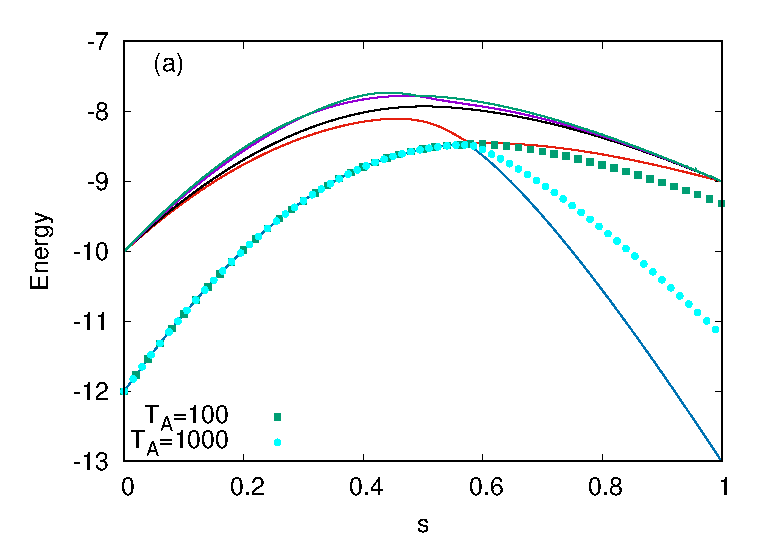
\includegraphics[scale=0.8 ]{63_O_g2.eps}
  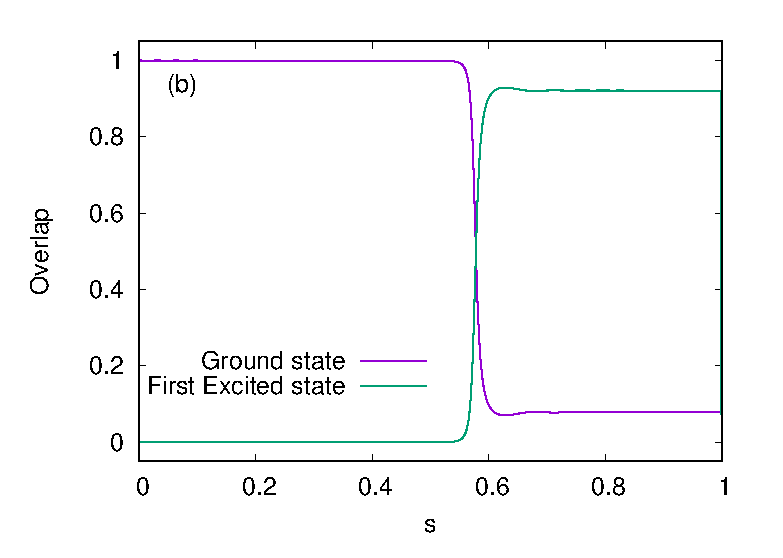
\includegraphics[scale=0.8 ]{63_Orig_Overlap.eps}
  \caption{For original Hamiltonian in Problem 63:  [Top] The energy spectra and instantaneous energy expectation values corresponding to $T_A$=100, and $T_A$=1000. [Bottom] The instantaneous overlap of the system state with the three lowest lying energy levels of the Hamiltonian for $T_A$=100.} 
   \label{fig:a52}
 \end{figure}

Figure~(\ref{fig:a54}(b)) makes it clear that the system state for $T_A$=100 starts to deviate from the ground state around the first energy anti-crossing. The amplitude shifted to the first excited state immediately transits to the second excited state, and further to the higher excited states. At the second anti-crossing, all of the remaining amplitude of the wave function in the ground state shifts to the first excited state, making the amplitude in the ground state drop to zero. This is suggestive of the fact that the minimum energy gap indeed closes at this point, making it a point of crossing between these energy levels. Another probable point of crossing between these levels occurs around $s$=0.465, causing all the amplitude present in the first excited state to transit to the ground state of the Hamiltonian. This results in an improved success probability.
\begin{figure}
\centering
  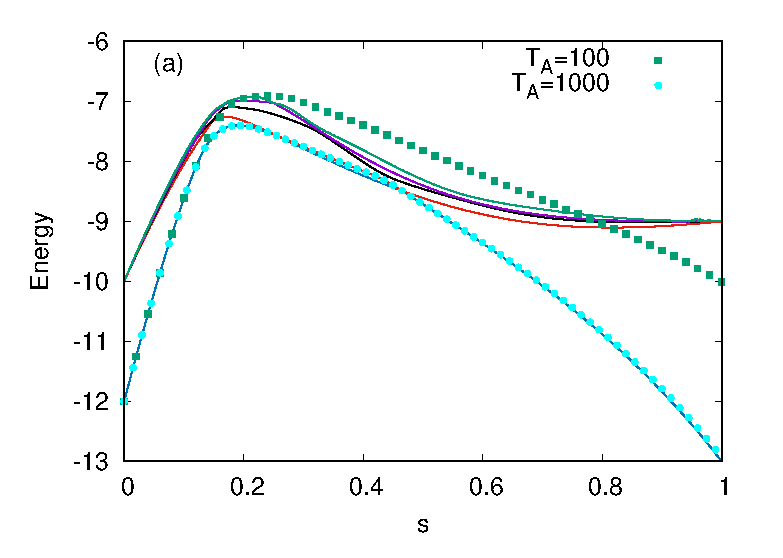
\includegraphics[scale=0.8 ]{63_A_g2.eps}  
\includegraphics[scale=0.8 ]{63_A_g2_Overlap.eps}
  \caption{After adding the antiferromagnetic Hamiltonian to Problem 63 (a): The energy spectra and instantaneous energy expectation values corresponding to $T_A$=100, and $T_A$=1000; (b): The overlap of the system state with the three lowest lying energy levels of the instantaneous Hamiltonian for $T_A$=100.}
    \label{fig:a54}
 \end{figure}

However, no such point of crossing was obtained while computing the minimum energy gaps for this case. This can be a consequence of the limited precision at which the energy spectrum of the time dependent Hamiltonian is computed. \begin{comment}As mentioned previously, the determination of minimum energy gaps is done employing the full diagonalization method, which requires too much resources (like time and storage)\end{comment}.\\

Additionally, as can be observed from Fig.~(\ref{fig:a54}), for $T_A$=1000 the system state shifts the full amplitude to the first excited state on reaching the first crossing. This amplitude then comes back to the ground state at the second crossing, explaining the increase in the success probability.\\
The mechanics of some of the other cases studied is shown in the appendix (see Figs. (\ref{fig:ap6} and \ref{fig:ap7} in the appendix).

Finally, Fig.~(\ref{fig:a46}) shows the success probability versus minimum energy gap plot for all the problems of the set, for the original Hamiltonian, and the Hamiltonian after adding the trigger. 

\begin{figure}
\centering 
\includegraphics[scale=0.8 ]{SuccVsGap_OA_g2.eps}
\caption{Success probability versus minimum energy gap for all the problems belonging to the set of 12-spin SAT problems, for annealing times 10, 100 an 1000, in the absence and presence of ferromagnetic trigger.}
\label{fig:a46}
\end{figure}

Upon adding the antiferromagnetic trigger with $g$=2, the scattering of the points of the curves increases compared to that of the original curves, as well as for the curves with the antiferromagnetic trigger with $g$=1 (see Fig.~(\ref{fig:a36})). This indicates that a larger number of problems have a non-adiabatic evolution in this case. This can be explained by narrowing of the minimum energy gaps, increase in the number of energy anti-crossings, and distortion of the energy spectra for a majority of the cases. Moreover, compared to Figs.~(\ref{fig:a18}) and (\ref{fig:a36}), the success probabilities after adding the trigger for $T_A$=10 are much smaller in this case. Lastly, the data points corresponding to the curves after adding the trigger, are not as limited to smaller values of the minimum gap, as there are more problems with an enlarged minimum energy gap in this case.\\

In summary, the consequences of adding the antiferromagnetic trigger are much more complicated than the effects of adding the ferromagnetic trigger, where the minimum energy gaps and the success probabilities always improve after adding the trigger.
\end{document}